% Requires the official AIAA/Overleaf `new-aiaa.cls` file to compile.
\documentclass[conf]{new-aiaa}

\usepackage[utf8]{inputenc}
\usepackage{textcomp}
\usepackage{graphicx}
\usepackage{amsmath}
\usepackage{amssymb}
\usepackage{booktabs}
\usepackage{longtable,tabularx}
\usepackage{subcaption}
\usepackage{siunitx}
\usepackage{url}
\usepackage{array}
\usepackage{float}
\usepackage[section]{placeins}

\setlength\LTleft{0pt}

\title{Integrated Propeller-Architecture Screening, Blown-Wing High-Lift Sizing, and Motor-Height Sensitivity for a \SI{5}{kg}-Class Distributed-Propulsion Aircraft}

\author{Nolan Nguyen\footnote{AA146 Capstone Team, Stanford University, Student Researcher.} and Codex Technical Collaborator\footnote{Automated analysis, scripting, and documentation support for aerodynamic trade studies.}}
\affil{AA146 Capstone, Stanford University, Stanford, California, 94305}

\begin{document}
\maketitle

\begin{abstract}
This paper documents the present end-to-end state of a blown-wing design workflow developed for a \SI{5}{kg}-class distributed-propulsion aircraft. The project begins with a fast Stage~1 Pareto-front optimizer that screens propeller count, propeller diameter, pitch ratio, and coarse propeller family while solving operating RPM internally. The resulting shortlist is then carried into a fixed-span geometry refinement, a rectangular-wing control-surface sizing study, a motor-height sensitivity study, and a representative motor/ESC target-sheet generator. The work is motivated primarily by two recent blown-wing studies. Hawkswell et al. demonstrated that a low-order, uniform two-dimensional jet model captures the first-order behaviour of a blown wing so long as the wing remains immersed in the jet, and further showed that propeller position and jet size govern the onset of abrupt stall.\cite{Hawkswell2022} Agrawal et al. experimentally characterized a blown slotted-flap wing in terms of section $c_l$, $c_x$, and $c_m$ as functions of angle of attack, flap angle, motor-axis angle, and jet momentum-excess coefficient, and showed that aggressive blown high-lift systems can achieve very large section lift while also incurring strong pitching-moment and stall-shape penalties.\cite{Agrawal2019} These two papers motivate the present modeling split: the blown portion of the wing is treated as a jet-covered two-dimensional strip, but aircraft-level $C_L$ and $C_M$ are always assembled by area-weighting blown and unblown portions of the wing at common $\alpha$. The current Stage~1 sweep evaluates 1386 propulsion architectures, of which 34 satisfy the present feasibility constraints and 11 survive onto the Pareto front. The selected study concept, referred to throughout as rank~6, is a $10\times 5.5\times 2.2$~in balanced propeller arrangement that was retained because it sits near the low-cruise-power edge of the nondominated set while also preserving the highest blown-wing momentum coefficient in the screened family. The downstream control-surface study indicates that the present concept supports a large, overlap-aware inboard single-slotted flap and a viable outboard aileron, but still falls short of the \SI{4.0}{m/s} target low-speed condition once the common-$\alpha$ whole-wing lift curve is used. The motor-height trade produces the expected three-part trend: lift first improves as immersion is recovered, then saturates, then degrades as the motor is dropped too far and the modeled stall becomes more abrupt. The full repository structure, equations, plots, and findings are recorded here in implementation-matched form so that future work can replace the current surrogates with experimentally calibrated or CFD-calibrated relationships without losing the logic of the present design space exploration.
\end{abstract}

\section*{Nomenclature}
\begin{longtable*}{@{}ll@{}}
\(A_{\mathrm{disk}}\) & total propeller disk area \\
\(AR\) & wing aspect ratio \\
\(b\) & wing span \\
\(c\) & wing chord \\
\(c_f\) & flap chord \\
\(c_a\) & aileron chord \\
\(C_D\) & aircraft drag coefficient referenced to freestream dynamic pressure \\
\(C_L\) & aircraft lift coefficient referenced to freestream dynamic pressure \\
\(C_M\) & aircraft pitching-moment coefficient referenced to freestream dynamic pressure \\
\(c_d, c_l, c_m\) & local two-dimensional section coefficients \\
\(C_\mu\) & wing-reference momentum coefficient used in the Stage~1 surrogate \\
\(\Delta c_J\) & jet momentum-excess coefficient used in Agrawal et al. \\
\(D_p\) & propeller diameter \\
\(e\) & Oswald efficiency factor \\
\(h/c\) & nondimensional jet or motor height parameter \\
\(J\) & propeller advance ratio \\
\(m\) & aircraft mass \\
\(N_p\) & number of propellers \\
\(P/D\) & propeller pitch ratio \\
\(q_\infty\) & freestream dynamic pressure \\
\(q_b\) & local dynamic pressure in the blown strip \\
\(S\) & wing planform area \\
\(S_b, S_u\) & blown and unblown wing areas \\
\(T\) & thrust \\
\(V_\infty\) & freestream velocity \\
\(V_{\mathrm{eff}}\) & effective blown velocity over the blown wing strip \\
\(v_i\) & induced velocity from actuator-disk theory \\
\(\alpha\) & angle of attack \\
\(\delta_f\) & flap deflection angle \\
\(\delta_m\) & motor-axis angle \\
\(\lambda\) & wing taper ratio \\
\(\rho\) & air density \\
\end{longtable*}

\section{Introduction}

The present project addresses a classic blown-wing design problem under unusually tight geometric constraints. The aircraft span is fixed at \SI{2.0}{m}, the low-speed operating point is set at \SI{4.0}{m/s}, the cruise operating point is set at \SI{10.0}{m/s}, and the gross design mass target is \SI{5.0}{kg}. These conditions immediately imply a demanding freestream-referenced lift requirement. Using the rectangular baseline wing of span \(b=\SI{2.0}{m}\) and chord \(c=\SI{0.35}{m}\), the freestream dynamic pressure at \SI{4}{m/s} is only about \SI{9.8}{Pa}; the corresponding freestream-referenced aircraft lift requirement is
\begin{equation}
C_{L,\mathrm{req}} = \frac{W}{q_\infty S} \approx 7.15,
\end{equation}
which is far beyond conventional unblown wing capability. The design task is therefore not to make a mildly assisted wing, but to identify a propulsion architecture and high-lift system that can make a very-low-speed blown wing credible without producing unreasonable cruise penalties.

The workflow implemented in this repository was built to answer four questions in sequence:
\begin{enumerate}
\item Which propeller architectures are energetically attractive once geometric packing, thrust, and blown-lift constraints are enforced?
\item Which architecture should be carried forward into more detailed wing and control-surface work?
\item What flap, aileron, and motor-height choices are consistent with a blown slotted-flap concept once the wing is treated as a mixture of blown and unblown regions?
\item What operating-point implications follow for motor selection, trim burden, and low-speed controllability?
\end{enumerate}

The present repository therefore combines a coarse Pareto-front architecture screener with more detailed follow-on studies. The philosophy is deliberately hierarchical: use a simple but broad Stage~1 optimizer to downselect the propeller family, then impose literature-backed blown-wing physics on a smaller set of architectures. This is the same general spirit seen in Hawkswell et al., who used low-order reasoning to explore the coupled role of propeller size, position, and wing immersion in the jet before optimizing more specific aircraft-level outcomes,\cite{Hawkswell2022} and in Agrawal et al., who emphasized fitting section response surfaces from test data rather than pretending that one single momentum-theory equation captures every aspect of a blown flap.\cite{Agrawal2019}

\section{Literature Basis and Modeling Philosophy}

\subsection{Hawkswell et al.: jet immersion, finite jet size, and propeller placement}

Hawkswell et al. are the primary motivation for the present motor-height and blown-strip modeling strategy.\cite{Hawkswell2022} Three findings from that paper are central.

First, they show that the wing must remain within the propeller jet across the relevant operating range. Their wording is unusually direct: if the wing moves outside the jet, even slightly, the wing can stall suddenly.\cite{Hawkswell2022} That insight motivates the present repository's decision to model motor height primarily through a jet-immersion criterion rather than through an arbitrary empirical bonus factor.

Second, Hawkswell et al. demonstrate that a uniform two-dimensional actuator-disc treatment is an acceptable first-order approximation of the blown-wing problem so long as the main concern is first-order lift behaviour. They compared two-dimensional and three-dimensional actuator-disc variants and concluded that, provided the wing remains submerged in the jet, variations in jet height have only second-order effect on the overall lift distribution and peak lift.\cite{Hawkswell2022} This finding is why the present repository is comfortable treating the blown strip as a nominally uniform two-dimensional region even though the final wing is finite.

Third, Hawkswell et al. show that there is an important balance between jet size and jet velocity. A smaller propeller for fixed thrust increases jet velocity, which can steepen the lift response with flap angle; however, the smaller jet height also makes it easier for the jet to miss the wing, reducing the stall margin.\cite{Hawkswell2022} This balance is one of the main reasons Stage~1 does not simply minimize power or maximize jet velocity in isolation. The selected architecture must balance cruise power, induced blowing authority, and geometric coverage of the wing.

The same paper also provides practical motor-height scales that are used in the repository as anchors, not as exact fitted constants. Their idealized no-nacelle configuration found a favorable position near \(0.21c\) below the wing centerline, while the more practical nacelle-included analysis brought the favorable scale closer to \(0.12c\).\cite{Hawkswell2022} In the present code these values are treated as the main \emph{paper-derived} motor-height scales, while the precise surrogate coefficients around them remain \emph{paper-informed} or \emph{heuristic}.

\subsection{Agrawal et al.: section response, slotted flaps, pitching moment, and aggressive stall}

Agrawal et al. provide the strongest direct experimental foundation for the present flap and wing-only section-response interpretation.\cite{Agrawal2019} Their wind-tunnel model was instrumented to vary flap angle, motor-axis angle, blowing level, and motor height, and they reported response surfaces in terms of section \(c_l\), \(c_x\), and \(c_m\). That format is particularly important for this project because it clarifies that large blown-wing lift is fundamentally a \emph{section plus jet} effect before it is an aircraft-level \(C_L\) effect.

Two observations from Agrawal et al. directly influenced the current code.

The first is their experimental magnitude: section \(c_l\) values near 8--9 were observed at strong blowing levels and aggressive flap deflections.\cite{Agrawal2019} This motivated the current repository change from overinflated freestream-scaled section curves to capped, common-\(\alpha\) section curves whose magnitudes remain within the same order as the experimental paper.

The second is their discussion of pitch and stall behaviour. Agrawal et al. note that increasing blowing changes \(c_m\), and that the sign and magnitude of this change depend strongly on flap angle and angle of attack.\cite{Agrawal2019} They further note that the \(20^\circ\) motor-axis-angle case appears to stall more suddenly and more aggressively than the \(10^\circ\) case in the \(40^\circ\) flap configuration, which they interpret as earlier upper-surface separation because the jet must bend through a larger angle to remain attached.\cite{Agrawal2019} That insight directly motivates the present repository's \emph{over-drop stall penalty}: a second mechanism, separate from immersion, that is intended to capture the idea that an overly aggressive motor/jet geometry can sharpen stall even after the wing is fully immersed in the jet.

\subsection{What is paper-derived, paper-informed, and heuristic?}

The distinction between evidence levels matters in this project.

\begin{itemize}
\item \textbf{Paper-derived}: the most direct anchors are the need for jet immersion, the practical motor-height scale near \(0.12c\), the idealized motor-height scale near \(0.21c\), the validity of a uniform two-dimensional jet-covered strip as a first-order approximation, and the order-of-magnitude section lift values reported by Agrawal et al.\cite{Hawkswell2022,Agrawal2019}
\item \textbf{Paper-informed}: the existence of separate clean and flap branches in the motor-height trade, the use of an over-drop penalty that activates mainly near stall, and the interpretation that flap-aligned propeller coverage matters because the jet/flap interaction is central to the lift benefit.\cite{Hawkswell2022,Agrawal2019}
\item \textbf{Heuristic / to be calibrated}: the exact steepness of the immersion switch, the onset values for the over-drop penalty, the polynomial weighting of low-angle and near-stall slotted-flap gains, and the motor-targeting safety factors.
\end{itemize}

The present paper keeps this distinction explicit because the repository is intended as a design workflow, not as a claim that every coefficient has already been fully calibrated.

\section{Repository Workflow and Script Architecture}

The repository is organized around a sequence of stages that mirror the design questions listed earlier. Table~\ref{tab:scripts} summarizes the main files and their roles.

\begin{table*}[H]
\centering
\caption{Repository script architecture and the role of each main module.}
\label{tab:scripts}
\begin{tabularx}{\textwidth}{@{}>{\ttfamily}l X X@{}}
\toprule
File & Primary role & Commentary \\
\midrule
optimizer/core/data\_models.py & Mission assumptions and result schemas & Defines the global mass, voltage, geometry, aerodynamic, and sweep assumptions used by Stage~1 and downstream studies. \\
optimizer/core/physics.py & Stage~1 physics engine & Implements propeller surrogates, packing constraints, RPM solution, thrust and power calculation, blown-lift feasibility, and mass closure. \\
optimizer/core/mass\_model.py & Mass fits & Converts required propeller, motor, ESC, and battery loads into estimated masses using representative local datasets. \\
optimizer/core/pareto.py & Nondominated filter & Extracts the Pareto front from the feasible Stage~1 results. \\
optimizer/stages/stage1\_screen.py & Stage~1 runner & Evaluates the full architecture sweep and writes the main screening CSVs. \\
optimizer/stages/stage2\_prop\_span.py & Prop-layout handoff & Converts Stage~1 nondominated points into explicit prop-center and packing reports. \\
optimizer/core/stage3\_refinement.py & Fixed-span geometry refinement & Runs the AeroSandbox-based wing and tail geometry refinement around shortlisted propulsion architectures. \\
optimizer/stages/stage3\_aerosandbox.py & Stage~3 runner & Writes the fixed-span geometry refinement results and plot artifacts. \\
optimizer/core/airfoil\_polar\_comparison.py & Airfoil comparison engine & Builds paper-style section response surfaces and representative wing-level airfoil comparisons. \\
optimizer/stages/airfoil\_polar\_comparison.py & Airfoil comparison runner & Generates the S1210, NACA~2412, and E423 comparison artifacts. \\
optimizer/core/high\_lift\_model.py & Shared blown high-lift model & Contains slotted-flap corrections, Cambridge-style immersion, and the over-drop penalty used by multiple downstream studies. \\
optimizer/core/control\_surface\_sizing.py & Rectangular wing control study & Sizes the inboard slotted flap and outboard aileron, builds whole-wing $C_L$ and $C_M$ curves, and reports low-speed aileron proxies. \\
optimizer/stages/control\_surface\_sizing.py & Control-surface runner & Writes the rectangular-wing control artifacts for a selected rank. \\
optimizer/core/motor\_height\_trade.py & Motor-height sensitivity study & Evaluates clean and flapped branches over a range of motor drops using immersion plus over-drop stall penalty. \\
optimizer/stages/motor\_height\_trade.py & Motor-height runner & Writes the motor-height summary CSVs and plots. \\
optimizer/core/motor\_targeting.py & Representative motor/ESC target sheet & Converts the selected architecture operating point into Kv, current, power, and class-level motor/ESC targets. \\
optimizer/stages/motor\_targeting.py & Motor-target runner & Writes the motor target summary and the class-comparison plot. \\
optimizer/stages/validate\_outputs.py & Output consistency check & Ensures that the generated CSV schemas and expected artifacts remain coherent after code changes. \\
\bottomrule
\end{tabularx}
\end{table*}

This script architecture is not incidental; it embodies the philosophy of the project. Stage~1 is intentionally broad and cheap. The later files are narrower and more physically specific, but they only run after the architecture space has been pruned. This is the computational analogue of the design logic argued by Hawkswell et al.: use low-order reasoning to understand the main architectural trade before investing in more expensive analysis.\cite{Hawkswell2022}

\section{Stage~1 Pareto-Front Propeller Optimizer}

\subsection{Design space and fixed assumptions}

The Stage~1 optimizer screens the architecture space listed in Table~\ref{tab:stage1-space}. All values in this table come directly from the current implementation in \texttt{optimizer/core/data\_models.py}.

\begin{table}[H]
\centering
\caption{Stage~1 screened architecture space.}
\label{tab:stage1-space}
\begin{tabular}{@{}ll@{}}
\toprule
Parameter & Values \\
\midrule
Propeller count \(N_p\) & \(4, 6, 8, 10, 12, 14, 16\) \\
Diameter \(D_p\) [in] & \(4.0, 4.5, 5.0, 5.5, 6.0, 6.5, 7.0, 7.5, 8.0, 9.0, 10.0\) \\
Pitch ratio \(P/D\) & \(0.40, 0.50, 0.60, 0.70, 0.80, 0.90\) \\
Propeller family & high\_thrust, balanced, cruise \\
\bottomrule
\end{tabular}
\end{table}

The current global mission assumptions used by the optimizer are:
\begin{align}
m &= \SI{5.0}{kg}, &
b &= \SI{2.0}{m}, &
c &= \SI{0.35}{m}, \\
V_{\mathrm{low}} &= \SI{4.0}{m/s}, &
V_{\mathrm{cruise}} &= \SI{10.0}{m/s}, &
t_{\mathrm{loiter}} &= \SI{18}{min}.
\end{align}
The pack voltage is fixed at \SI{14.8}{V} and the baseline rectangular wing area is \(S=bc=\SI{0.70}{m^2}\).

\subsection{Propeller and blowing surrogate}

The Stage~1 propulsion model remains a surrogate, but it is internally consistent. The current thrust and shaft power relations are
\begin{align}
T_{\mathrm{per}} &= C_T \rho n^2 D_p^4, \\
P_{\mathrm{shaft,per}} &= C_P \rho n^3 D_p^5,
\end{align}
where \(n=\mathrm{RPM}/60\) and \(C_T\) and \(C_P\) are taken from coarse propeller-family fits. The purpose of these fits is not to identify a final propeller, but to keep the Stage~1 optimizer broad enough to search the architecture space quickly.

The total effective blown velocity is then obtained from an actuator-disc interpretation:
\begin{align}
v_i &= \sqrt{\frac{T_{\mathrm{tot}}}{2\rho A_{\mathrm{disk}}}}, \\
V_{\mathrm{eff}} &= V_\infty + 2v_i.
\end{align}
Stage~1 also defines a wing-reference momentum coefficient,
\begin{equation}
C_\mu = \frac{T_{\mathrm{tot}}}{q_\infty S},
\end{equation}
which is later used as one measure of blown authority.

The choice to keep both \(V_{\mathrm{eff}}\) and \(C_\mu\) in the optimizer is directly motivated by Hawkswell et al. Their discussion of jet size versus jet velocity implies that one cannot rank architectures purely by thrust, purely by power, or purely by jet speed: the candidate must also preserve enough jet coverage to keep the wing immersed.\cite{Hawkswell2022}

\subsection{Area-weighted blown-wing feasibility}

The main low-speed feasibility question in Stage~1 is not whether the unblown wing can fly at \SI{4}{m/s}; it clearly cannot. The question is whether the propeller architecture can create enough blown-strip dynamic pressure and blown-section capability to keep the working local \(c_l\) below a conservative ceiling.

The baseline Stage~1 low-speed model therefore divides the wing into unblown and blown regions and evaluates the required blown velocity from the remaining lift after the unblown region has done all it can. In simplified form,
\begin{equation}
L_{\mathrm{rem}} = W - q_\infty S_u c_{l,\mathrm{ceil}},
\end{equation}
and the required blown-strip dynamic pressure follows as
\begin{equation}
q_{b,\mathrm{req}} = \frac{L_{\mathrm{rem}}}{S_b c_{l,\mathrm{ceil}}}.
\end{equation}
The corresponding required effective blown velocity is
\begin{equation}
V_{\mathrm{eff,req}} = \sqrt{\frac{2q_{b,\mathrm{req}}}{\rho}}.
\end{equation}

This is not yet a full Agrawal-style \(\Delta c_J\) surface fit, but it serves the same design purpose: it forces the optimizer to ask how much local blown dynamic pressure is actually needed to carry the wing at the low-speed operating point, rather than presuming the answer in advance.\cite{Agrawal2019}

\subsection{Objectives and constraints}

The present Stage~1 Pareto front uses three objectives:
\begin{align}
\min \; P_{\mathrm{low}}, \qquad
\min \; E_{\mathrm{loiter}}, \qquad
\min \; m_{\mathrm{propulsion}}.
\end{align}

At the same time, the following constraints are enforced:
\begin{itemize}
\item propeller packing on the fixed \SI{2.0}{m} span, including fuselage clearance, inter-prop clearance, and tip margin,
\item low-speed \(V_{\mathrm{eff}} \ge V_{\mathrm{eff,req}}\),
\item positive thrust margin at low speed and cruise,
\item tip Mach margin,
\item disk-loading bounds,
\item mass budget closure.
\end{itemize}

The packing constraints are important. They prevent the optimizer from choosing impossible high-count, large-diameter combinations simply because they look attractive in a power-only model. This again reflects Hawkswell's point that propeller size and location are not independent and that the benefit of a smaller jet must be considered together with the wing's need to remain inside it.\cite{Hawkswell2022}

\section{Stage~1 Results and Selection of the Rank~6 Architecture}

\subsection{Screening outcome}

The current run of the repository evaluates 1386 architecture combinations. Of these, 34 are feasible under the present constraints and 11 remain on the nondominated Stage~1 front. The resulting design space is shown in Fig.~\ref{fig:stage1-pareto}. Two features are immediately visible.

First, the feasible set is strongly shaped by geometry. Many nominally attractive architectures disappear once the explicit fuselage clearance, inter-prop spacing, and tip margin are enforced. Second, the nondominated set does not collapse to a single propeller count. Instead, the front contains a family of four-, six-, eight-, and ten-propeller solutions that trade cruise power, low-speed power, and blown authority against one another.

\begin{figure}[H]
    \centering
    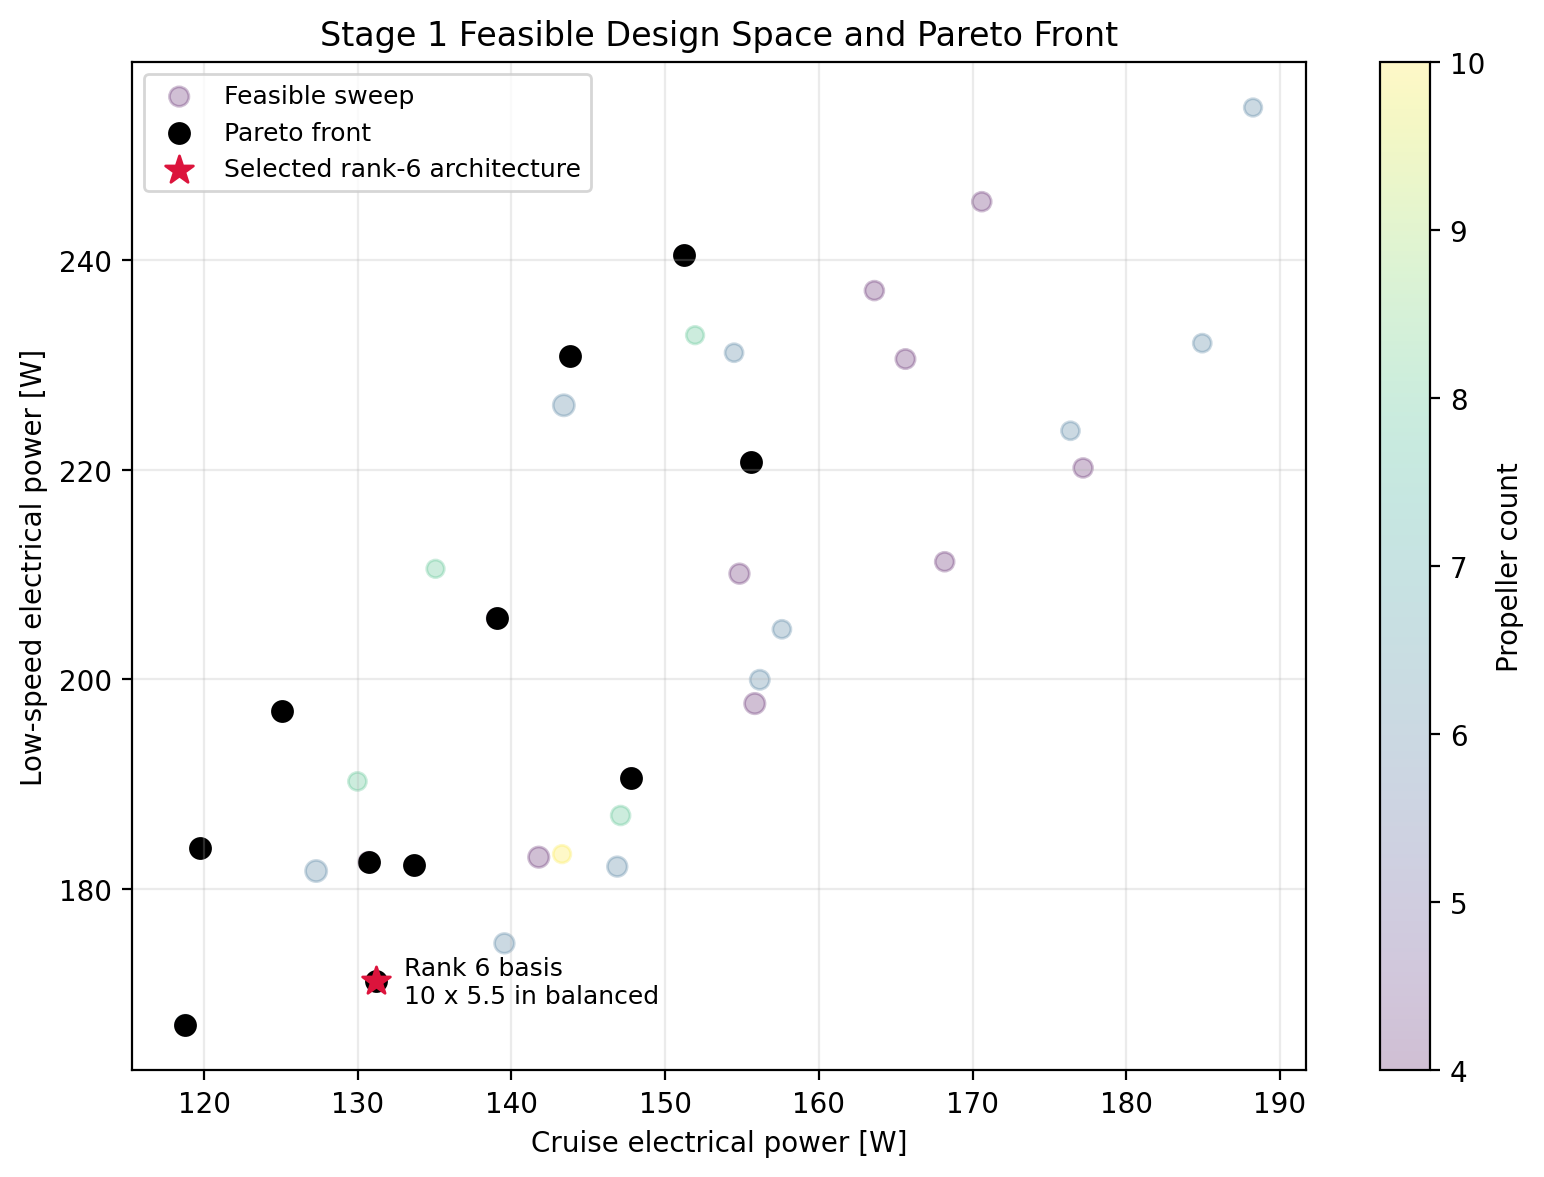
\includegraphics[width=0.92\linewidth]{../outputs/stage1_pareto_trade.png}
    \caption{Stage~1 feasible architecture space and Pareto front. Point color indicates propeller count. The selected rank~6 propulsion architecture is highlighted in red. The figure shows that the selected point is not an isolated optimum, but part of a broader nondominated family in which ten-propeller architectures occupy the low-power and high-coverage corner of the design space.}
    \label{fig:stage1-pareto}
\end{figure}

\subsection{Why rank~6 was selected}

The concept used throughout the downstream studies is the Stage~3 rank~6 propulsion architecture:
\begin{equation}
10 \times 5.5 \times 2.2 \;\text{in}, \qquad P/D = 0.40, \qquad \text{balanced prop family}.
\end{equation}

It is important to be precise about why this architecture was retained. It was not chosen because it had the single lowest cruise power in the Pareto set; the \(10\times 5.5\) cruise-family neighbor is slightly lower in cruise power. Instead, the \(10\times 5.5\) \emph{family} was retained because it sits very near the low-cruise-power edge while also delivering the highest Stage~1 momentum coefficient in the nondominated set:
\begin{equation}
C_\mu \approx 1.544,
\end{equation}
with
\begin{equation}
V_{\mathrm{eff}} \approx \SI{14.62}{m/s}.
\end{equation}
Within that family, the balanced propeller surrogate was carried forward because it preserved the same blown authority while reducing low-speed electrical power relative to the cruise-family variant.

In other words, the selected architecture was not intended to be the final global optimum over every downstream metric. It was selected because it was a strong \emph{blown-wing study vehicle}: low enough in cruise power to remain plausible for the mission, yet high enough in blown authority to give the downstream high-lift study a meaningful chance of success.

Figure~\ref{fig:stage1-authority} makes this logic explicit. The selected point does not maximize \(V_{\mathrm{eff}}\) in absolute terms; several four-propeller architectures produce higher jet velocity. However, those higher-\(V_{\mathrm{eff}}\) cases pay a substantial cruise-power penalty and, because of lower blown-span fraction, do not necessarily represent a more useful high-lift concept once the full wing is considered. The selected \(10\times 5.5\) architecture retains the highest momentum coefficient in the Pareto set while remaining close to the low-cruise-power boundary, which is precisely the compromise the project sought.

\begin{figure}[H]
    \centering
    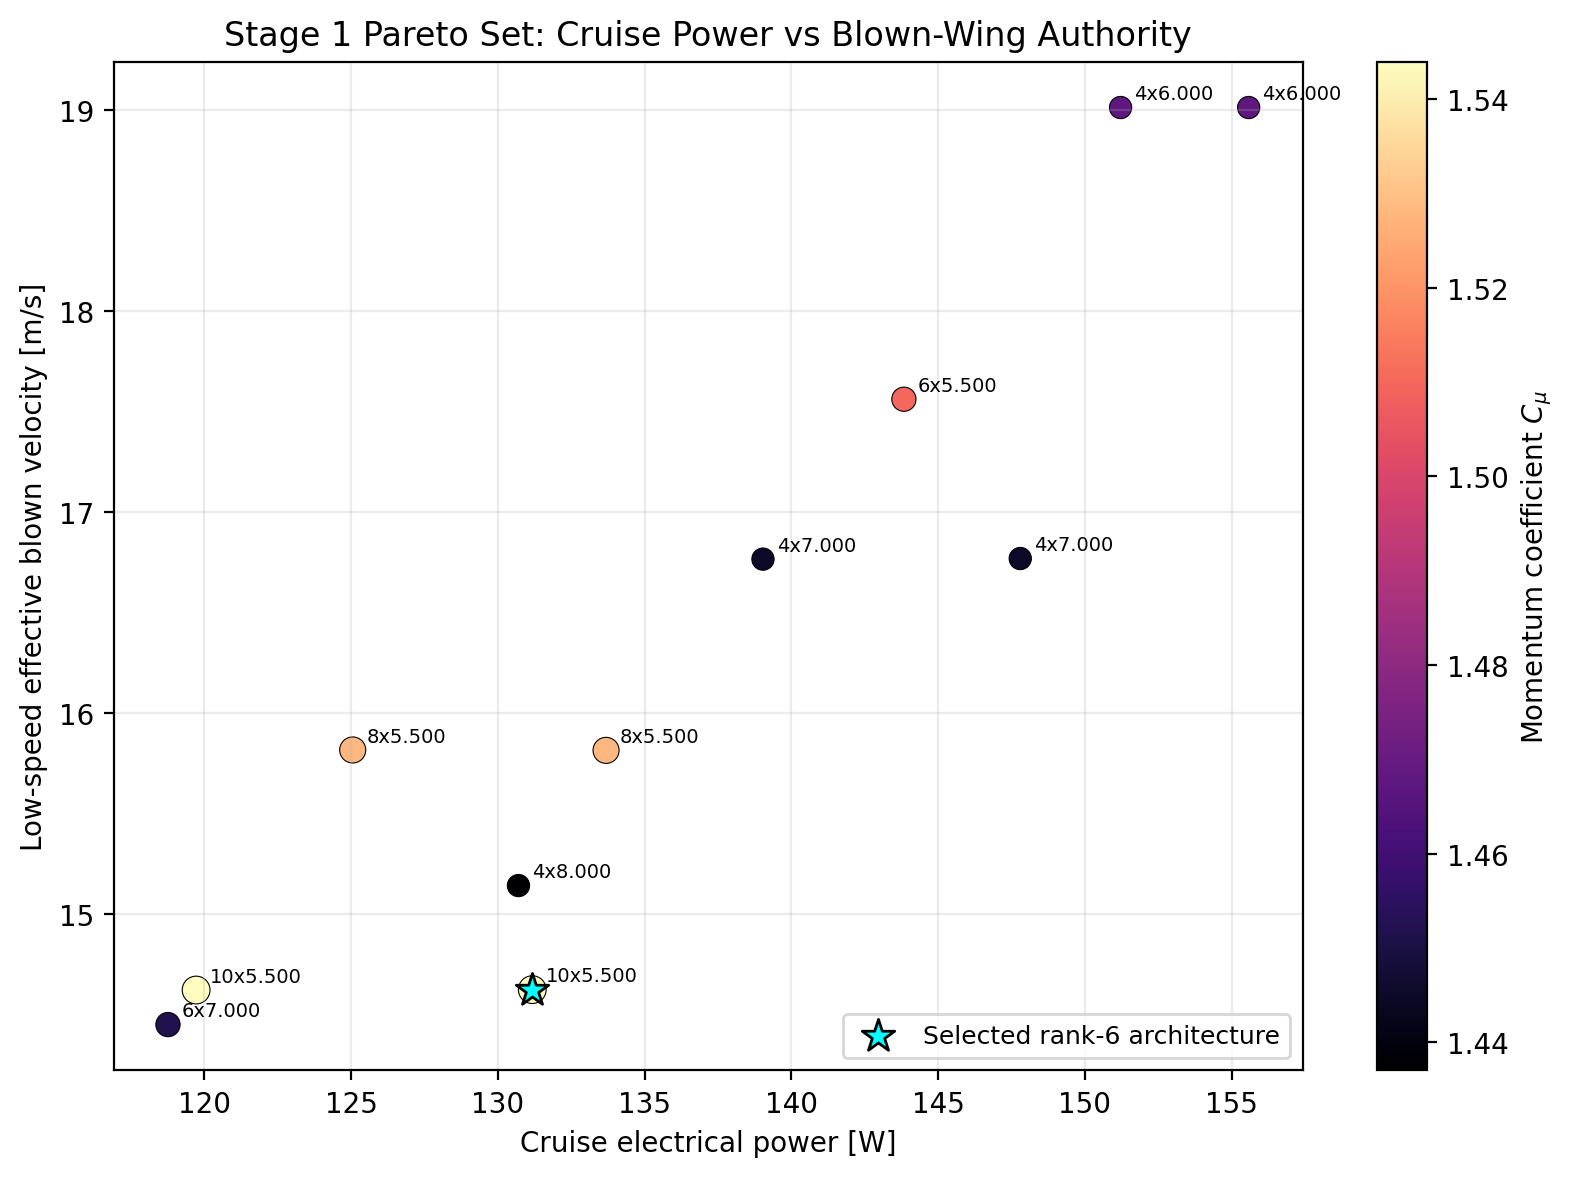
\includegraphics[width=0.92\linewidth]{../outputs/stage1_blown_authority_trade.png}
    \caption{Stage~1 Pareto set plotted in terms of cruise electrical power and low-speed blown-wing authority. Marker color indicates momentum coefficient \(C_\mu\). The selected rank~6 architecture does not deliver the maximum absolute \(V_{\mathrm{eff}}\), but it lies on the low-power side of the nondominated set while preserving the highest \(C_\mu\) in the screened family. This is the main rationale for carrying it forward.}
    \label{fig:stage1-authority}
\end{figure}

\subsection{Selected Stage~1 operating point}

The current Stage~1 values for the selected rank~6 architecture are:
\begin{align}
\mathrm{RPM}_{\mathrm{low}} &\approx 9696, &
\mathrm{RPM}_{\mathrm{cruise}} &\approx 9565, \\
P_{\mathrm{low}} &\approx \SI{171.2}{W}, &
P_{\mathrm{cruise}} &\approx \SI{131.2}{W}, \\
E_{\mathrm{loiter}} &\approx \SI{39.35}{Wh}, &
V_{\mathrm{eff}} &\approx \SI{14.62}{m/s}, \\
V_{\mathrm{eff,req}} &\approx \SI{9.47}{m/s}, &
C_\mu &\approx 1.544.
\end{align}
The present Stage~1 mass closure for this concept gives about \SI{0.11}{kg} of propulsion mass and \SI{0.29}{kg} of battery mass, resulting in a total built-mass estimate of about \SI{2.40}{kg} under the current fixed-system-mass assumption. This is a useful observation: the current configuration is not yet limited by the battery energy budget or propulsion mass budget. Instead, the main challenge remains high-lift performance at the \SI{4}{m/s} requirement.

\section{Airfoil Comparison and Wing-Section Direction}

Before sizing control surfaces, the repository compares three airfoils under a representative blown-wing scenario: S1210, NACA~2412, and E423. This study does not replace a full three-dimensional wing analysis, but it is useful for understanding the trade among lift, drag, and pitching moment before committing to a section family.

\begin{figure}[H]
    \centering
    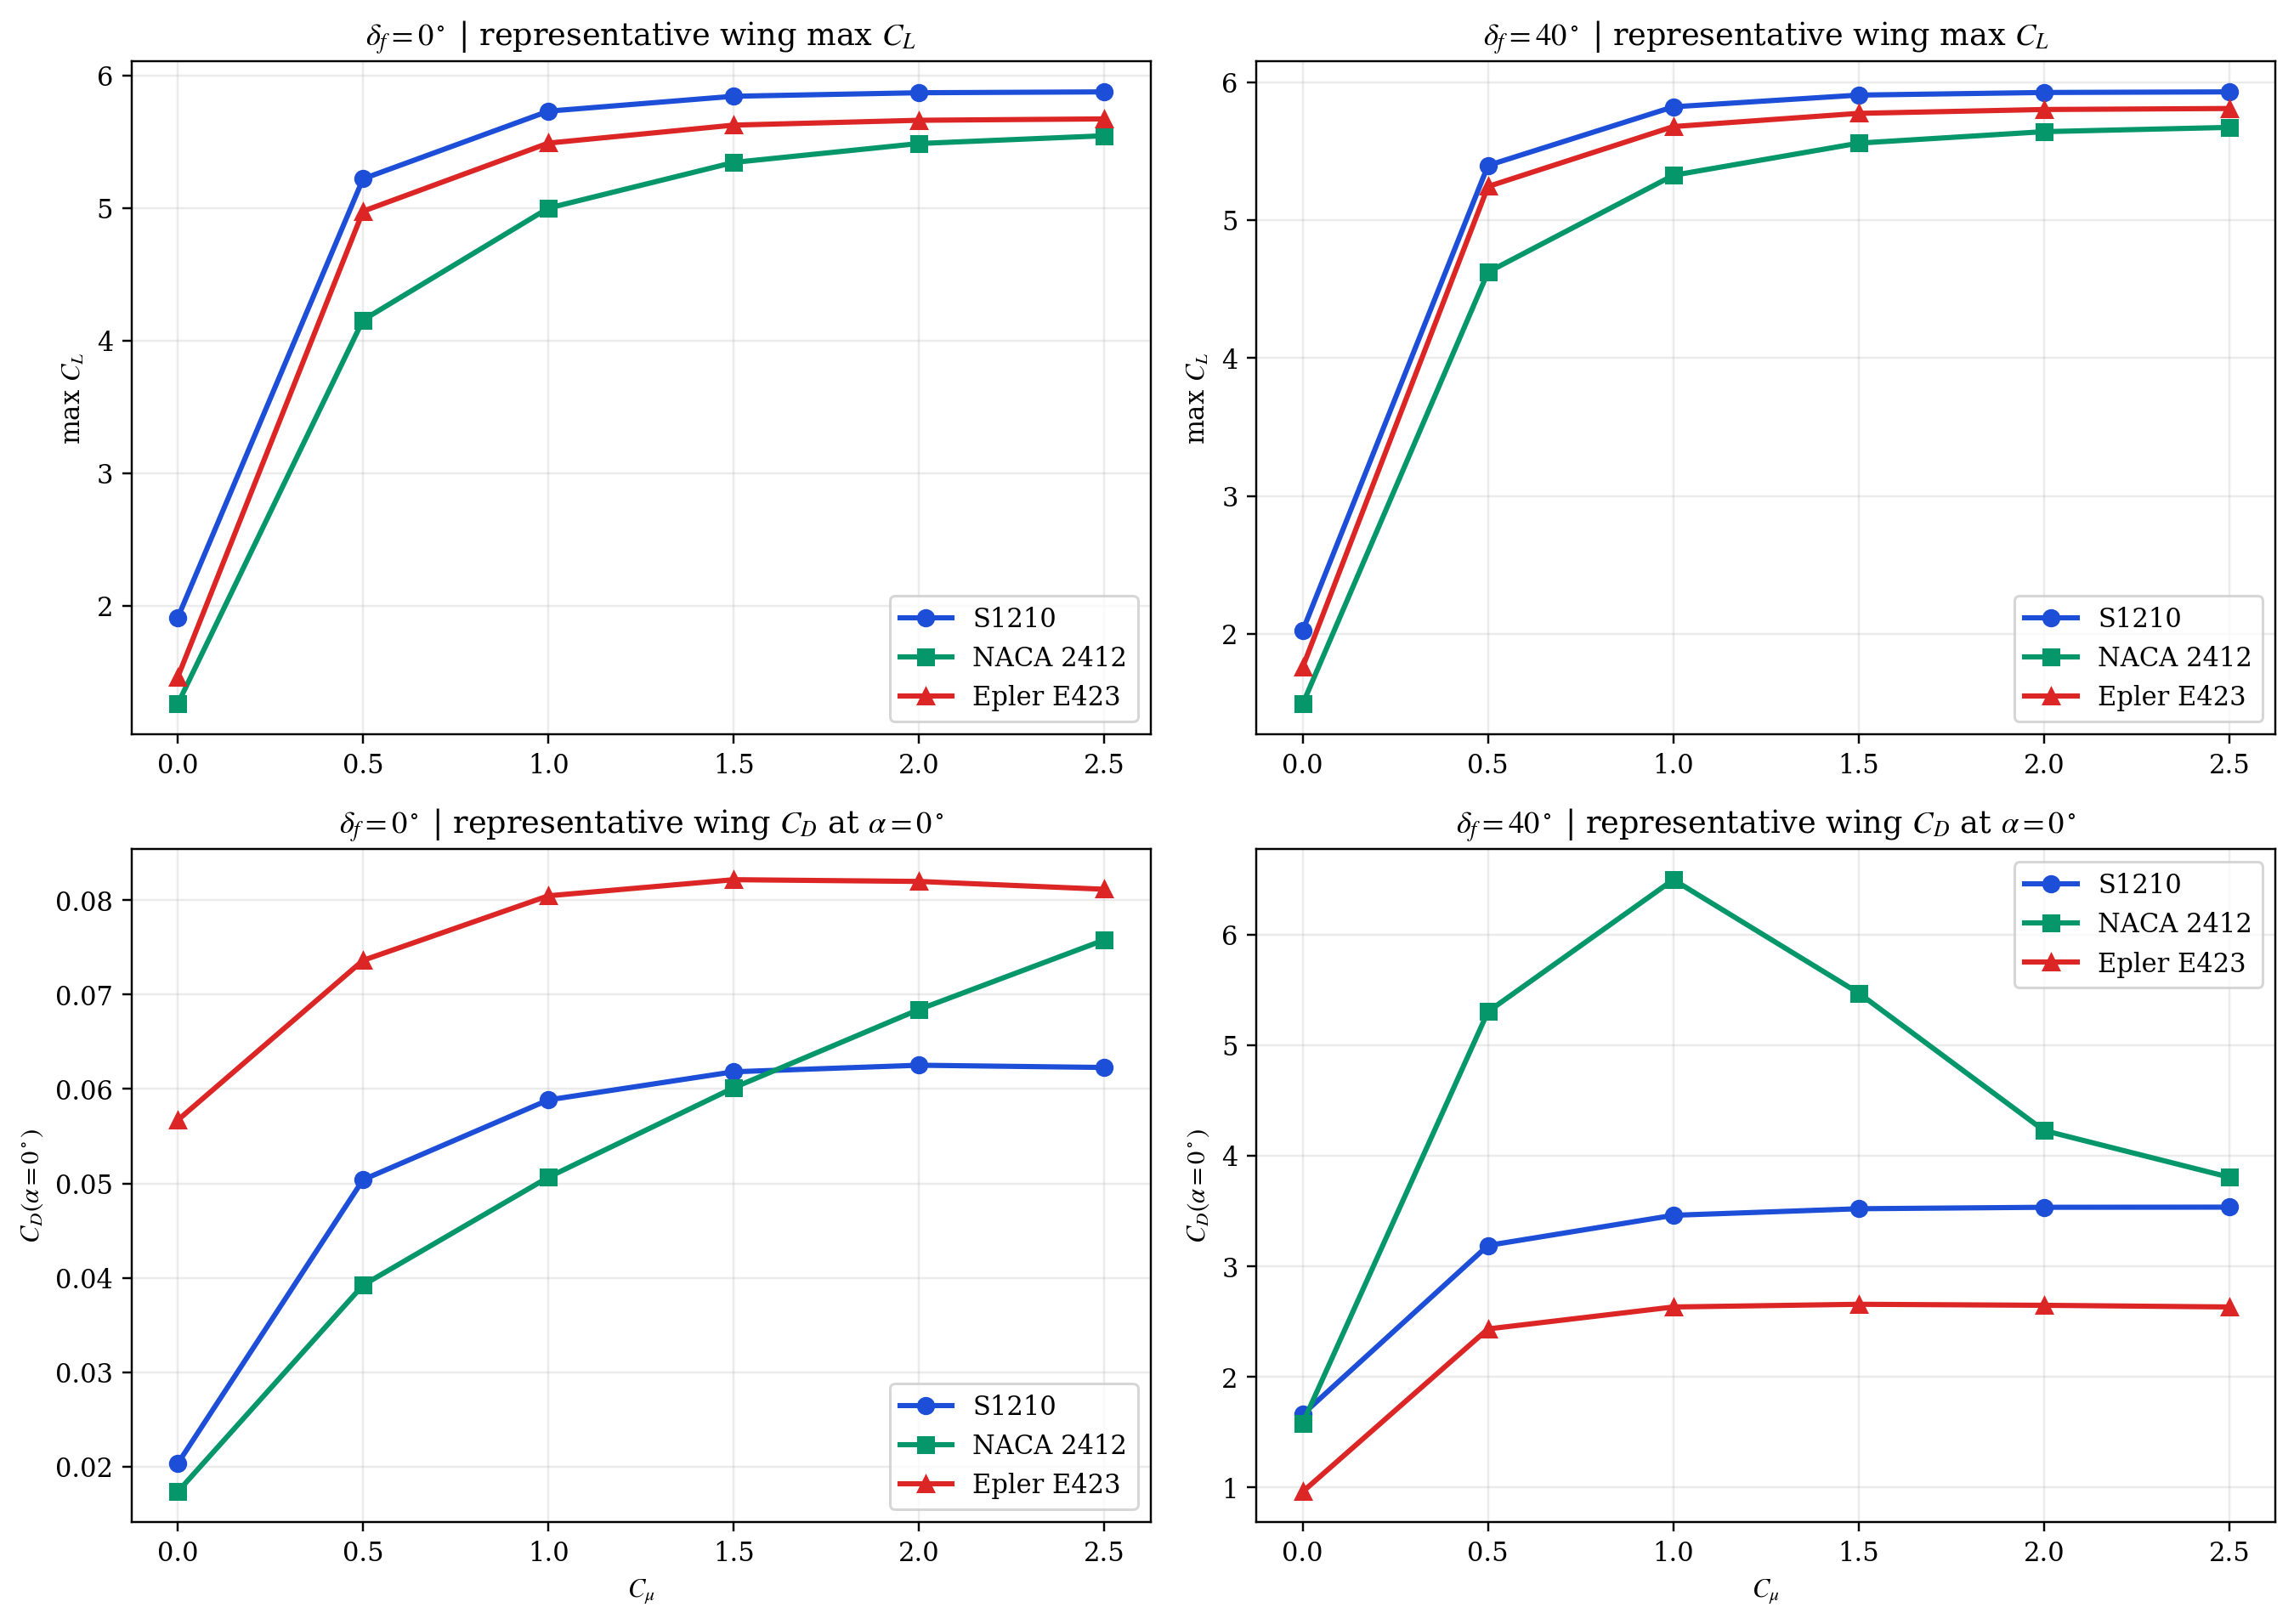
\includegraphics[width=0.92\linewidth]{../outputs/airfoil_comparison/airfoil_comparison_summary.png}
    \caption{Representative wing-level airfoil comparison under the current blown-wing assumptions. The S1210 and E423 sections both outperform NACA~2412 in achievable blown-wing lift, but they do so at the cost of more negative pitching moment. This is consistent with the central high-lift versus trim-burden trade observed in the control-surface study.}
    \label{fig:airfoil-summary}
\end{figure}

At \(\delta_f = 40^\circ\) and representative blowing level \(C_\mu=1.5\), the current wing-level summary predicts:
\begin{itemize}
\item S1210: \(C_{L,\max,\mathrm{rep}} \approx 5.91\), \(C_M(\alpha=0) \approx -0.82\),
\item E423: \(C_{L,\max,\mathrm{rep}} \approx 5.77\), \(C_M(\alpha=0) \approx -0.70\),
\item NACA~2412: \(C_{L,\max,\mathrm{rep}} \approx 5.56\), \(C_M(\alpha=0) \approx -0.37\).
\end{itemize}

This mirrors the design intuition behind the project. NACA~2412 is easier to live with from a trim perspective, but it gives up meaningful blown-wing lift. S1210 provides the strongest lift, but also the strongest nose-down tendency. E423 sits between the two. The present rectangular-wing study therefore uses S1210 not because it is uniquely superior in every metric, but because it gives the highest-lift edge in the current blown-wing envelope and is therefore a useful upper-bound wing section for the control-surface study. Agrawal et al. provide the physical context for this trade by showing that strong blown-flap systems couple high lift and nontrivial pitching-moment behaviour rather than improving one without affecting the other.\cite{Agrawal2019}

\section{Planform Refinement and Selected Geometry}

After the Stage~1 screen, the 11 nondominated architectures are carried into a fixed-span geometry refinement. This stage uses AeroSandbox to refine root chord, taper, washout, and control-surface placement while holding the propulsion architecture fixed. Although the remainder of this paper focuses on a rectangular wing for control-surface sizing --- per the later project constraint --- the Stage~3 refined planform is still informative because it indicates the geometric direction the solver prefers for the selected propulsion concept.

For the selected rank~6 concept, the current Stage~3 refined geometry is:
\begin{align}
S &\approx \SI{0.745}{m^2}, &
\lambda &\approx 0.62, &
\text{washout} &\approx -2.5^\circ.
\end{align}
The corresponding required blown velocity for the refined planform is reduced to about \SI{9.14}{m/s}, leaving a propulsor margin of about \SI{5.48}{m/s}. The top-view result is shown in Fig.~\ref{fig:rank6-topview}.

\begin{figure}[H]
    \centering
    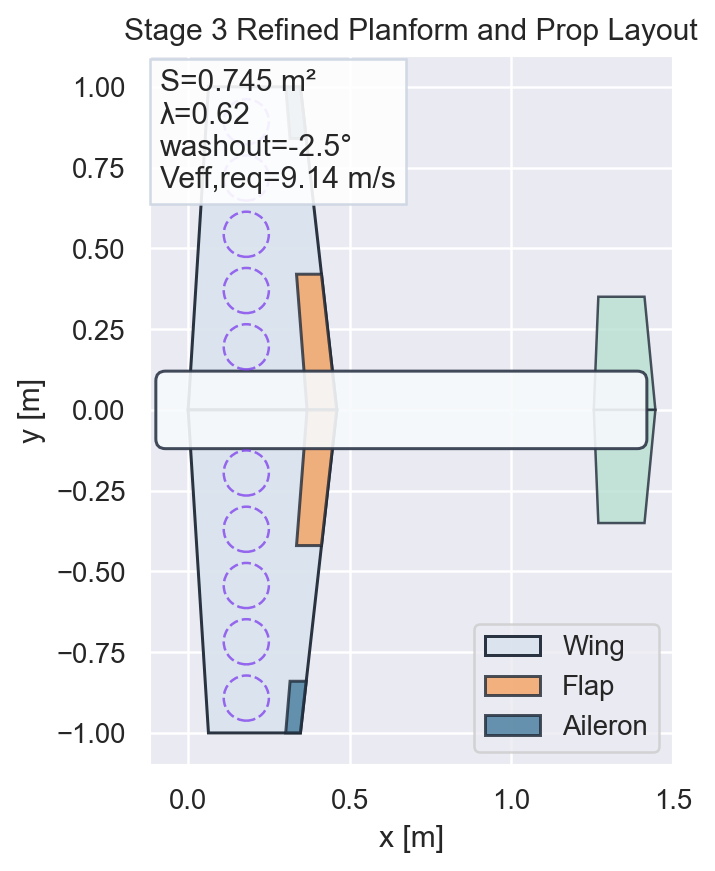
\includegraphics[width=0.72\linewidth]{../outputs/stage3_visuals/rank06_n10_d5p5_pd0p40_balanced_top_view.png}
    \caption{Stage~3 refined planform for the selected rank~6 propulsion concept. The refined geometry tends toward a moderate taper ratio and modest washout, indicating that the solver would prefer a somewhat larger and milder-tapered wing than the original rectangular baseline. The remainder of the present control-surface study nevertheless uses a rectangular wing because that geometric constraint was imposed explicitly for the current design phase.}
    \label{fig:rank6-topview}
\end{figure}

This distinction is important. The Stage~3 geometry result is best interpreted as a \emph{directional recommendation}, not as a final planform commitment. For the present design phase, the wing was deliberately constrained back to a rectangular box so that flap size, aileron size, and motor-flap alignment could be understood without the extra confounding effect of changing taper simultaneously.

\section{Rectangular-Wing Control-Surface Sizing}

\subsection{Why motors in front of flaps matter}

The present control-surface study focuses on a rectangular wing of span \SI{2.0}{m} and chord \SI{0.35}{m}. The specific design question is not merely ``what flap and aileron fit on the wing?'' but rather ``what flap and aileron make sense when the inboard propellers are intended to blow the flap system?''

Agrawal et al. provide the main physical motivation for this emphasis. Their section-response and wake results show that the blown slotted-flap system benefits from injecting higher total pressure into the flap region and turning the jet downward through the flap, thereby increasing lift while also modifying pitching moment.\cite{Agrawal2019} In other words, the flap is not an isolated high-lift device; it is part of a jet/flap system. That is why the present repository no longer allows the flap span to drift to the smallest-area solution. Instead, the flap candidates are penalized if they fail to cover enough of the inboard propeller array.

\subsection{Common-\(\alpha\) whole-wing assembly}

The repository now assembles the whole-wing lift and pitching-moment curves from blown and unblown regions at common \(\alpha\). In schematic form,
\begin{equation}
C_L(\alpha)
=
\frac{1}{q_\infty S}\sum_k q_k S_k c_{l,k}(\alpha),
\end{equation}
and similarly,
\begin{equation}
C_M(\alpha)
=
\frac{1}{q_\infty S c}\sum_k q_k S_k c_{m,k}(\alpha),
\end{equation}
where the index \(k\) spans the clean-unblown, clean-blown, flap-unblown, and flap-blown subareas. This is the crucial step that keeps the project from confusing a large section \(c_l\) with an equally large whole-wing \(C_L\).

The section polars themselves are built from three ingredients:
\begin{enumerate}
\item NeuralFoil-based clean and flap-deflected section response,
\item a staged slotted-flap correction that separates low-angle lift-curve displacement from near-stall augmentation,
\item the Cambridge-style blown-strip immersion weighting and the bounded over-drop stall penalty described later.
\end{enumerate}

\subsection{Selected flap and aileron geometry}

The current selected rectangular-wing control configuration is:
\begin{align}
\text{flap span fraction} &= 0.65 \; \text{of semispan}, \\
c_f/c &= 0.34, \\
\delta_f &= 40^\circ, \\
\text{aileron span fraction} &= 0.28 \; \text{of semispan}, \\
c_a/c &= 0.28.
\end{align}
The resulting layout is shown in Fig.~\ref{fig:layout}. The flap overlaps 8 of the 10 propeller disks, covers 80\% of the positive-half propeller centers, and covers about 60.3\% of the positive-half disk span. Those values are not arbitrary: they are the consequence of enforcing the idea that a blown-flap concept should put most of its inboard blowing over the flap, not over an unflapped region.

\begin{figure}[H]
    \centering
    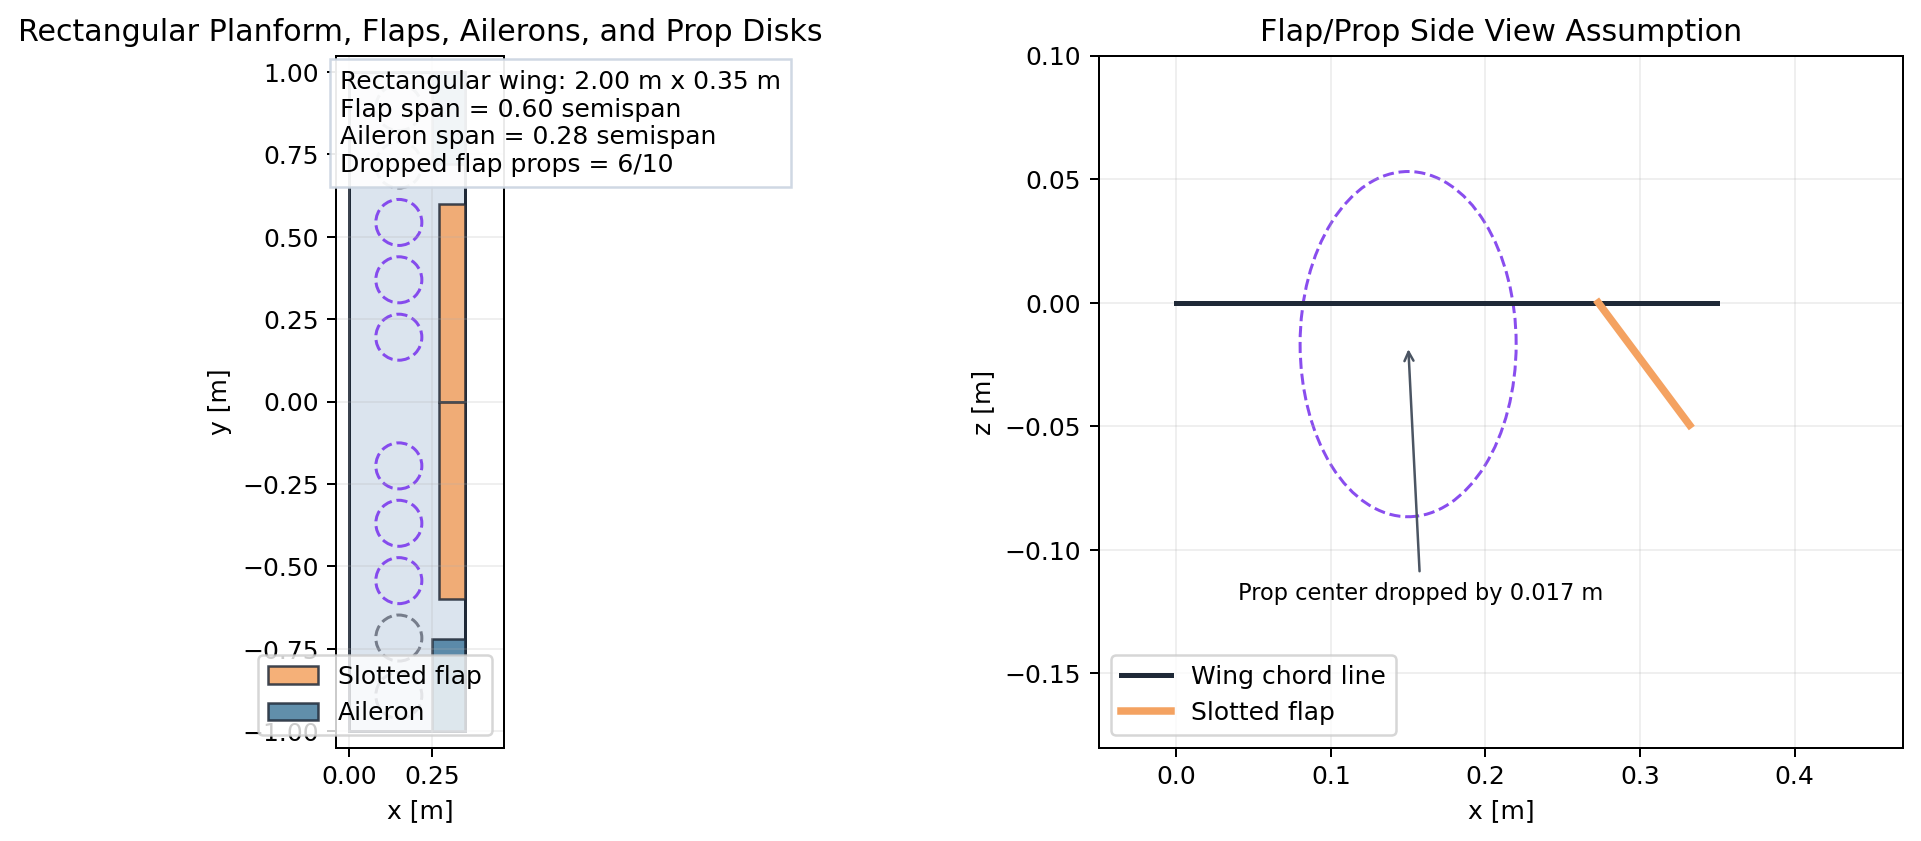
\includegraphics[width=0.92\linewidth]{../outputs/control_surface_sizing/rank06_n10_d5p5_p2p2_balanced_b3/layout.png}
    \caption{Rectangular-wing flap and aileron layout for the selected rank~6 propulsion architecture. The flap was intentionally pushed to \(65\%\) of semispan so that most of the inboard propeller disks lie over the slotted flap rather than over the clean wing. This geometry is a direct response to the blown-flap mechanism emphasized by Agrawal et al.\cite{Agrawal2019}}
    \label{fig:layout}
\end{figure}

The flap-sizing heatmap in Fig.~\ref{fig:flap-heatmap} shows why this solution was retained. Once overlap penalties are added, the best flap no longer lies at the smallest-area end of the design space. Instead, the favorable region shifts toward larger flap spans and larger flap chord ratios because the geometry must now satisfy the physical requirement that the jet and flap interact over a substantial portion of the span.

\begin{figure}[H]
    \centering
    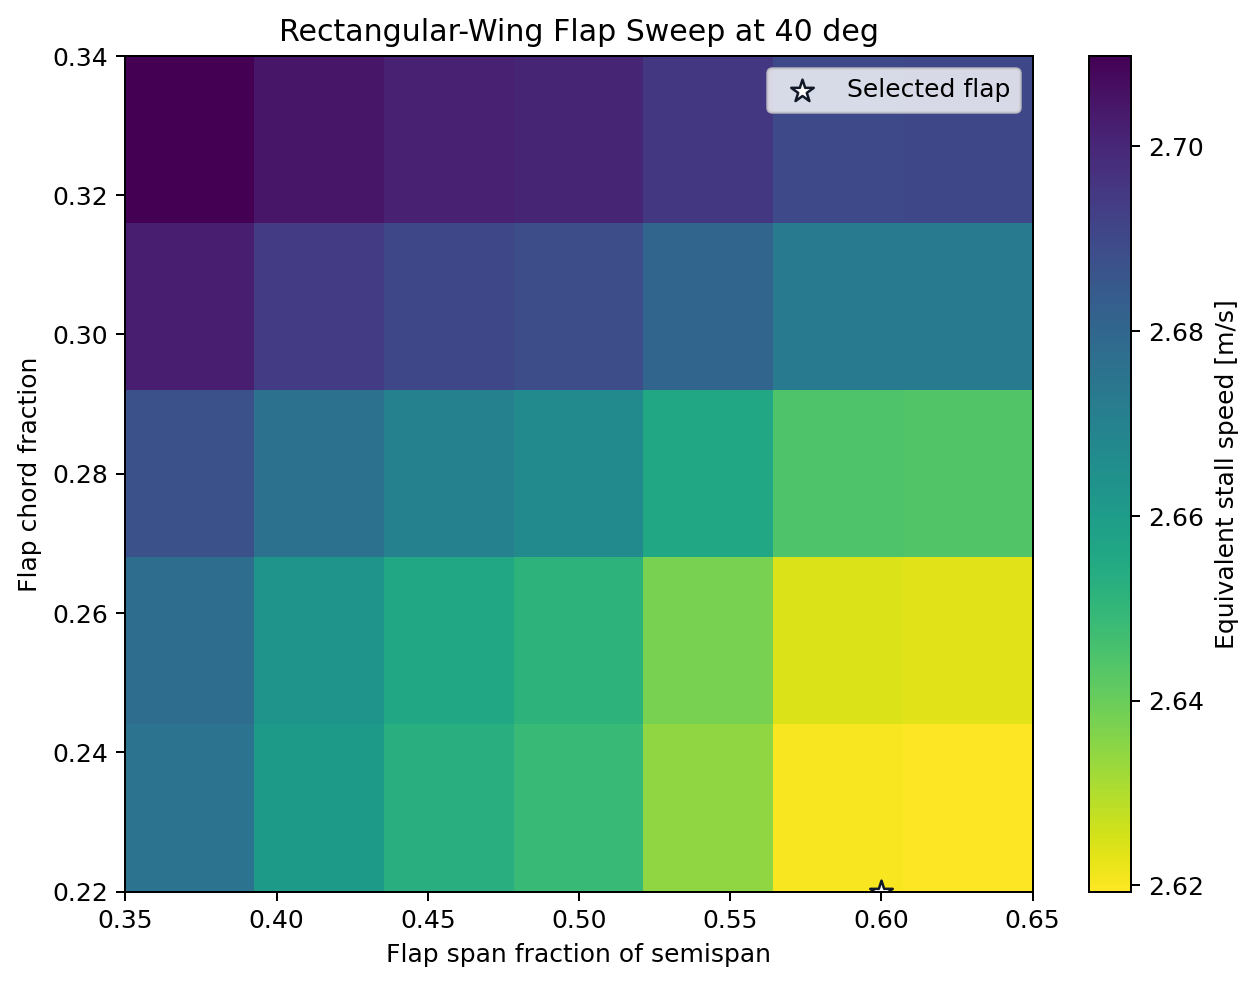
\includegraphics[width=0.92\linewidth]{../outputs/control_surface_sizing/rank06_n10_d5p5_p2p2_balanced_b3/flap_heatmap.png}
    \caption{Rectangular-wing flap heatmap for the selected rank~6 propulsion architecture. Once motor-overlap penalties are included, the optimum flap shifts toward the large-span, large-chord corner rather than collapsing to a small flap.}
    \label{fig:flap-heatmap}
\end{figure}

\subsection{Whole-wing \(C_L\), \(C_M\), and low-speed aileron authority}

The corrected whole-wing lift result for the selected rectangular wing is shown in Fig.~\ref{fig:total-cl}. The maximum freestream-referenced aircraft lift coefficient is
\begin{equation}
C_{L,\max} \approx 6.00,
\end{equation}
occurring at
\begin{equation}
\alpha \approx 13.27^\circ.
\end{equation}
This corresponds to an equivalent stall speed of about \SI{4.36}{m/s}. The \SI{4.0}{m/s} requirement line remains above the curve, meaning that the present rectangular blown-flap concept still falls short of the mission requirement once the whole wing is assembled consistently.

\begin{figure}[H]
    \centering
    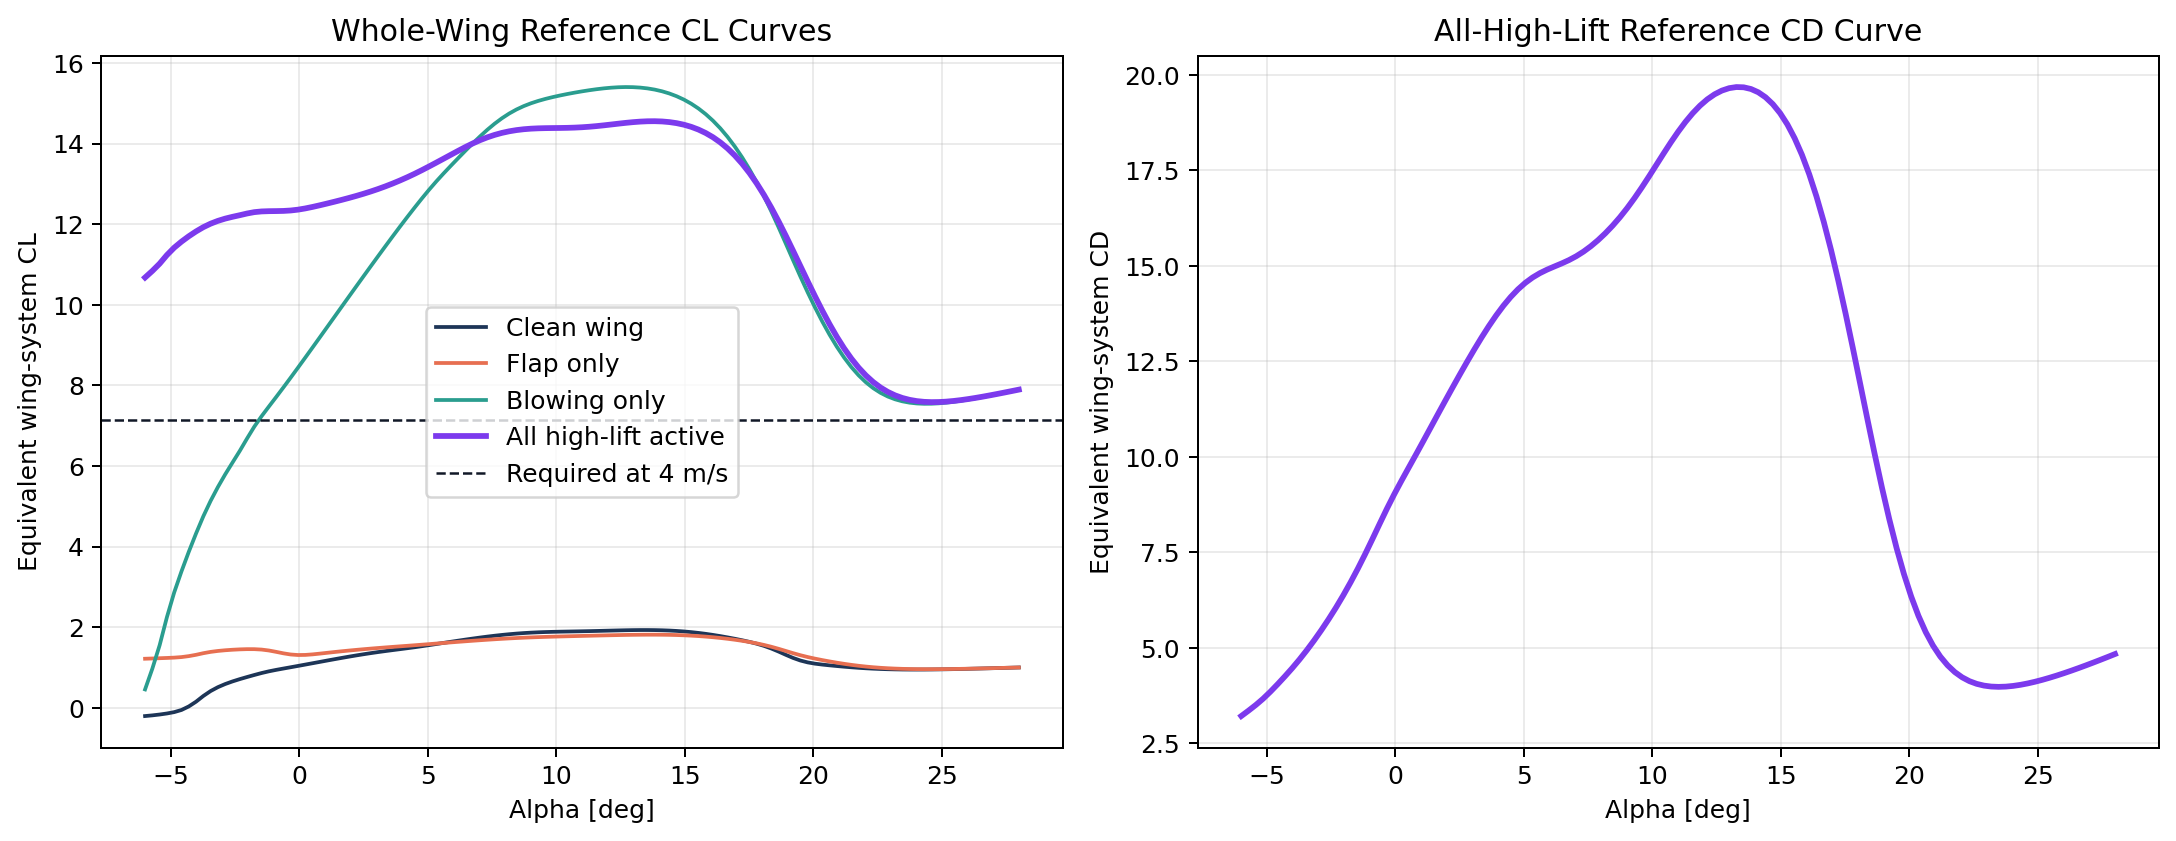
\includegraphics[width=0.92\linewidth]{../outputs/control_surface_sizing/rank06_n10_d5p5_p2p2_balanced_b3/total_cl_curve.png}
    \caption{Whole-wing freestream-referenced \(C_L\) curve for the selected rectangular-wing configuration. The all-high-lift branch includes flap deflection, blowing, and immersion weighting. The dashed lines denote the required freestream-referenced \(C_L\) at several flight speeds; the \SI{4.0}{m/s} line remains above the attainable value, demonstrating that the current concept is close but not yet sufficient for the original low-speed requirement.}
    \label{fig:total-cl}
\end{figure}

The pitching-moment consequence of this configuration is shown in Fig.~\ref{fig:total-cm}. At the same high-lift point,
\begin{equation}
C_M \approx -0.90,
\end{equation}
while the corresponding blowing-only branch is closer to \(C_M \approx -0.50\). This is a central result of the present project: the flap and the motors in front of it do add lift, but they also deepen the wing-only nose-down pitching moment. That trend is entirely consistent with Agrawal et al., who observed that blowing at nonzero flap angles can strongly alter \(c_m\) because the downward turning jet effectively acts through the flap system aft of the quarter chord.\cite{Agrawal2019}

\begin{figure}[H]
    \centering
    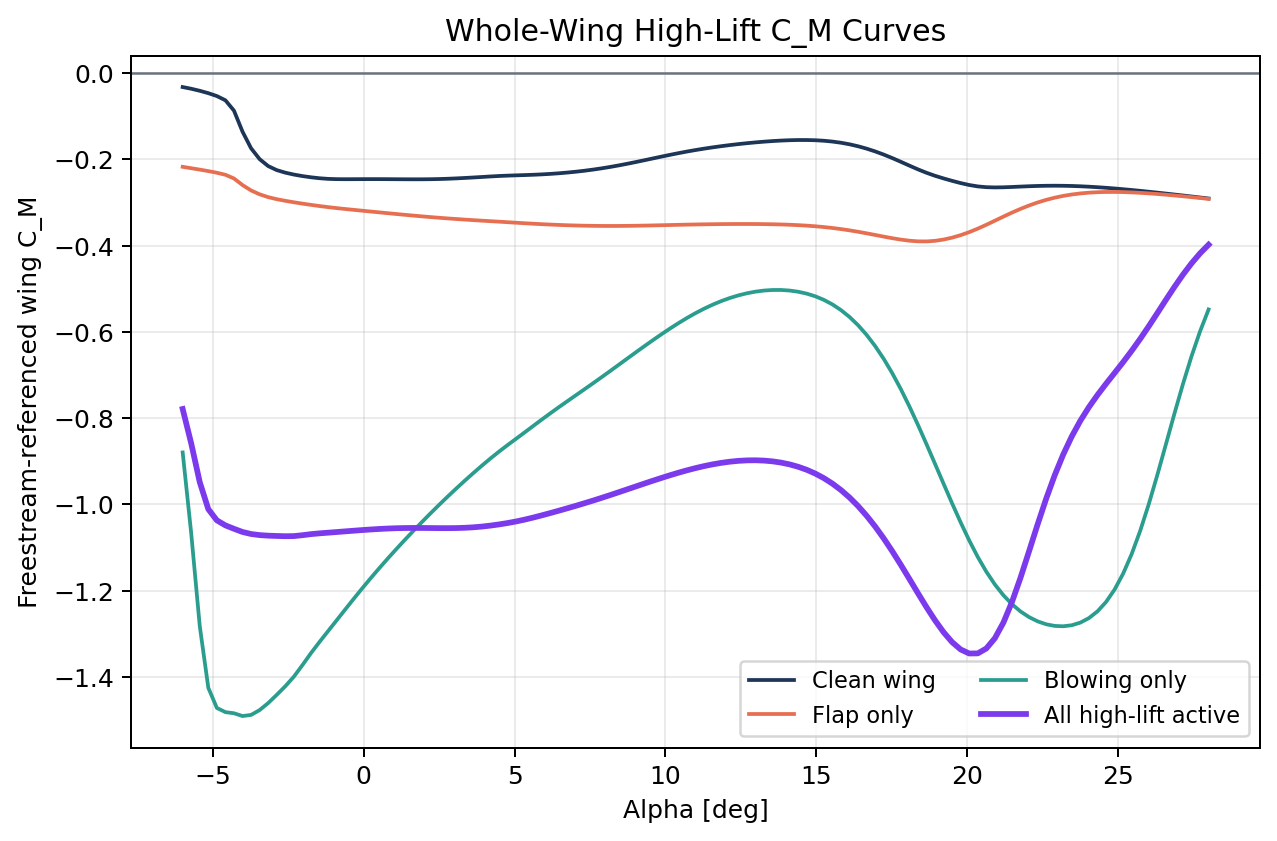
\includegraphics[width=0.92\linewidth]{../outputs/control_surface_sizing/rank06_n10_d5p5_p2p2_balanced_b3/total_cm_curve.png}
    \caption{Whole-wing freestream-referenced \(C_M\) curve for the selected rectangular-wing configuration. The flap-plus-blowing branch is substantially more nose-down than the blowing-only branch near the peak-lift condition, demonstrating that the blown slotted-flap system should be viewed as both a lift device and a trim device.}
    \label{fig:total-cm}
\end{figure}

The low-speed aileron proxy, shown in Fig.~\ref{fig:low-speed-aileron}, indicates that approximately 59\% of the aileron span lies in the blown intervals, with a local dynamic-pressure ratio of about 8.3 and a local effective velocity of about \SI{11.53}{m/s}. This produces a low-speed roll-rate proxy of approximately \SI{13}{deg/s} at the nominal \(14^\circ\) aileron deflection. This is not yet a full lateral-directional trim calculation, but it is a useful wing-only check that the blown inboard system does not completely destroy outboard control authority at low speed.

\begin{figure}[H]
    \centering
    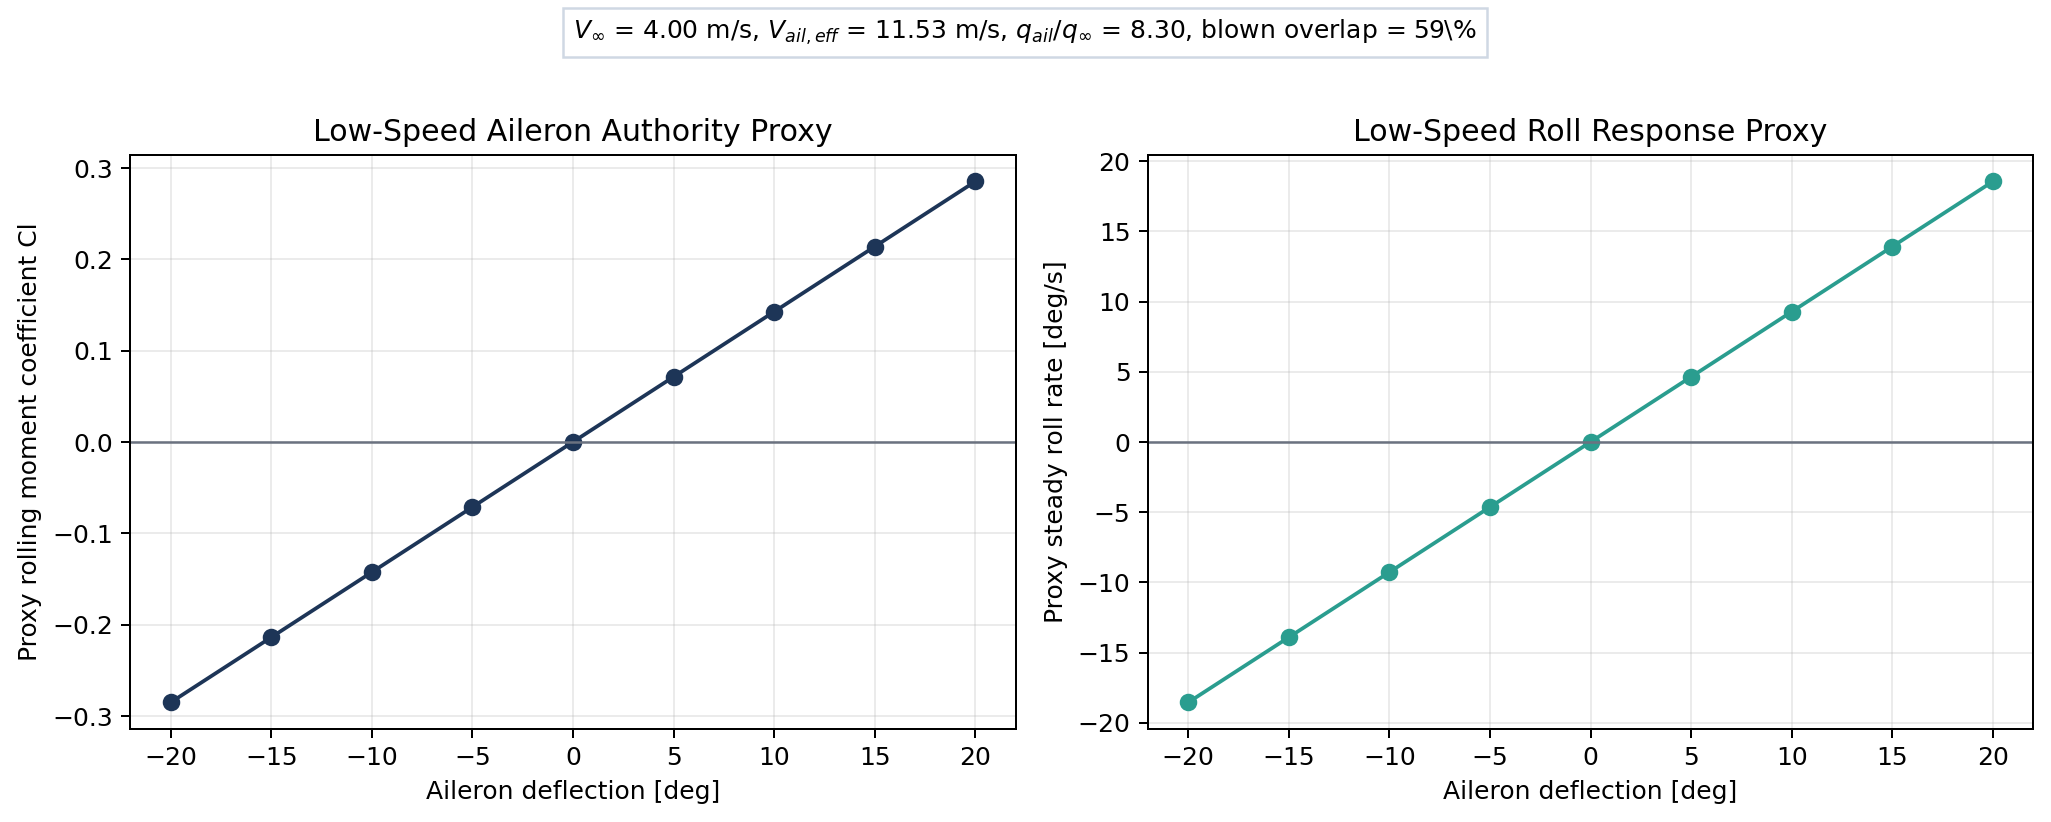
\includegraphics[width=0.92\linewidth]{../outputs/control_surface_sizing/rank06_n10_d5p5_p2p2_balanced_b3/low_speed_aileron_curves.png}
    \caption{Low-speed aileron authority proxy for the selected rectangular-wing configuration. The present model scales the aileron response by blown-span overlap and local dynamic pressure rather than claiming a full blown-control CFD solution. The result is nevertheless sufficient to show that the outboard aileron retains nonzero authority in the low-speed blown-wing condition.}
    \label{fig:low-speed-aileron}
\end{figure}

\section{Motor Height Trade: Clean Wing Versus Slotted-Flap Wing}

\subsection{Immersion and over-drop penalty}

The present motor-height trade combines two mechanisms.

The first is the Cambridge-style immersion criterion. In the code this is implemented as a smooth immersion factor that tends toward unity when the wing remains within the jet and tends toward zero when the jet rises above the wing. This is the direct implementation of Hawkswell et al.'s central observation that the wing should remain submerged in the jet at the operating incidence.\cite{Hawkswell2022}

The second is a bounded over-drop penalty. This is \emph{not} a paper-derived formula; it is a paper-informed surrogate introduced to capture the qualitative MIT/Agrawal-style observation that overly aggressive jet geometry can make the high-lift system stall more suddenly.\cite{Agrawal2019} The penalty is intentionally weak at low angle of attack and becomes active mainly near the peak-lift and post-stall region.

\subsection{Trade setup}

The motor-height study holds the selected rank~6 propulsion architecture, flap geometry, and aileron geometry fixed while sweeping
\begin{equation}
\frac{\Delta z_p}{c} \in \{0.00, 0.04, 0.08, 0.12, 0.16, 0.20, 0.24\}.
\end{equation}
Two scenario branches are evaluated:
\begin{enumerate}
\item a clean blown wing with no flap deployed,
\item a slotted flap plus blowing.
\end{enumerate}

This split is important because the present project does not assume that the no-flap and flap cases respond identically to motor height. Agrawal et al. strongly suggest otherwise by showing that the flap, motor-axis angle, and blowing level interact in the stall behaviour itself.\cite{Agrawal2019}

\subsection{Motor-height results}

The results of the trade are shown in Figs.~\ref{fig:motor-metrics} and \ref{fig:motor-overlay}. Both branches show the same three-stage behaviour:
\begin{enumerate}
\item too high: insufficient immersion, reduced blown benefit,
\item moderate drop: recovered immersion, near-optimal lift,
\item too low: over-drop penalty activates, stall sharpens, benefit degrades.
\end{enumerate}

For the clean blown wing, the best equivalent stall speed occurs near a drop of \SI{42}{mm} (\(\Delta z_p/c = 0.12\)) and the blown-wing benefit saturates by about \(\Delta z_p/c = 0.08\). For the slotted-flap branch, the optimum is similarly near \(\Delta z_p/c = 0.12\), but the degradation beyond that point is somewhat more gradual. This is physically plausible: the flap system can tolerate somewhat more jet immersion before the upper-surface or post-flap flow begins to deteriorate.

\begin{figure}[H]
    \centering
    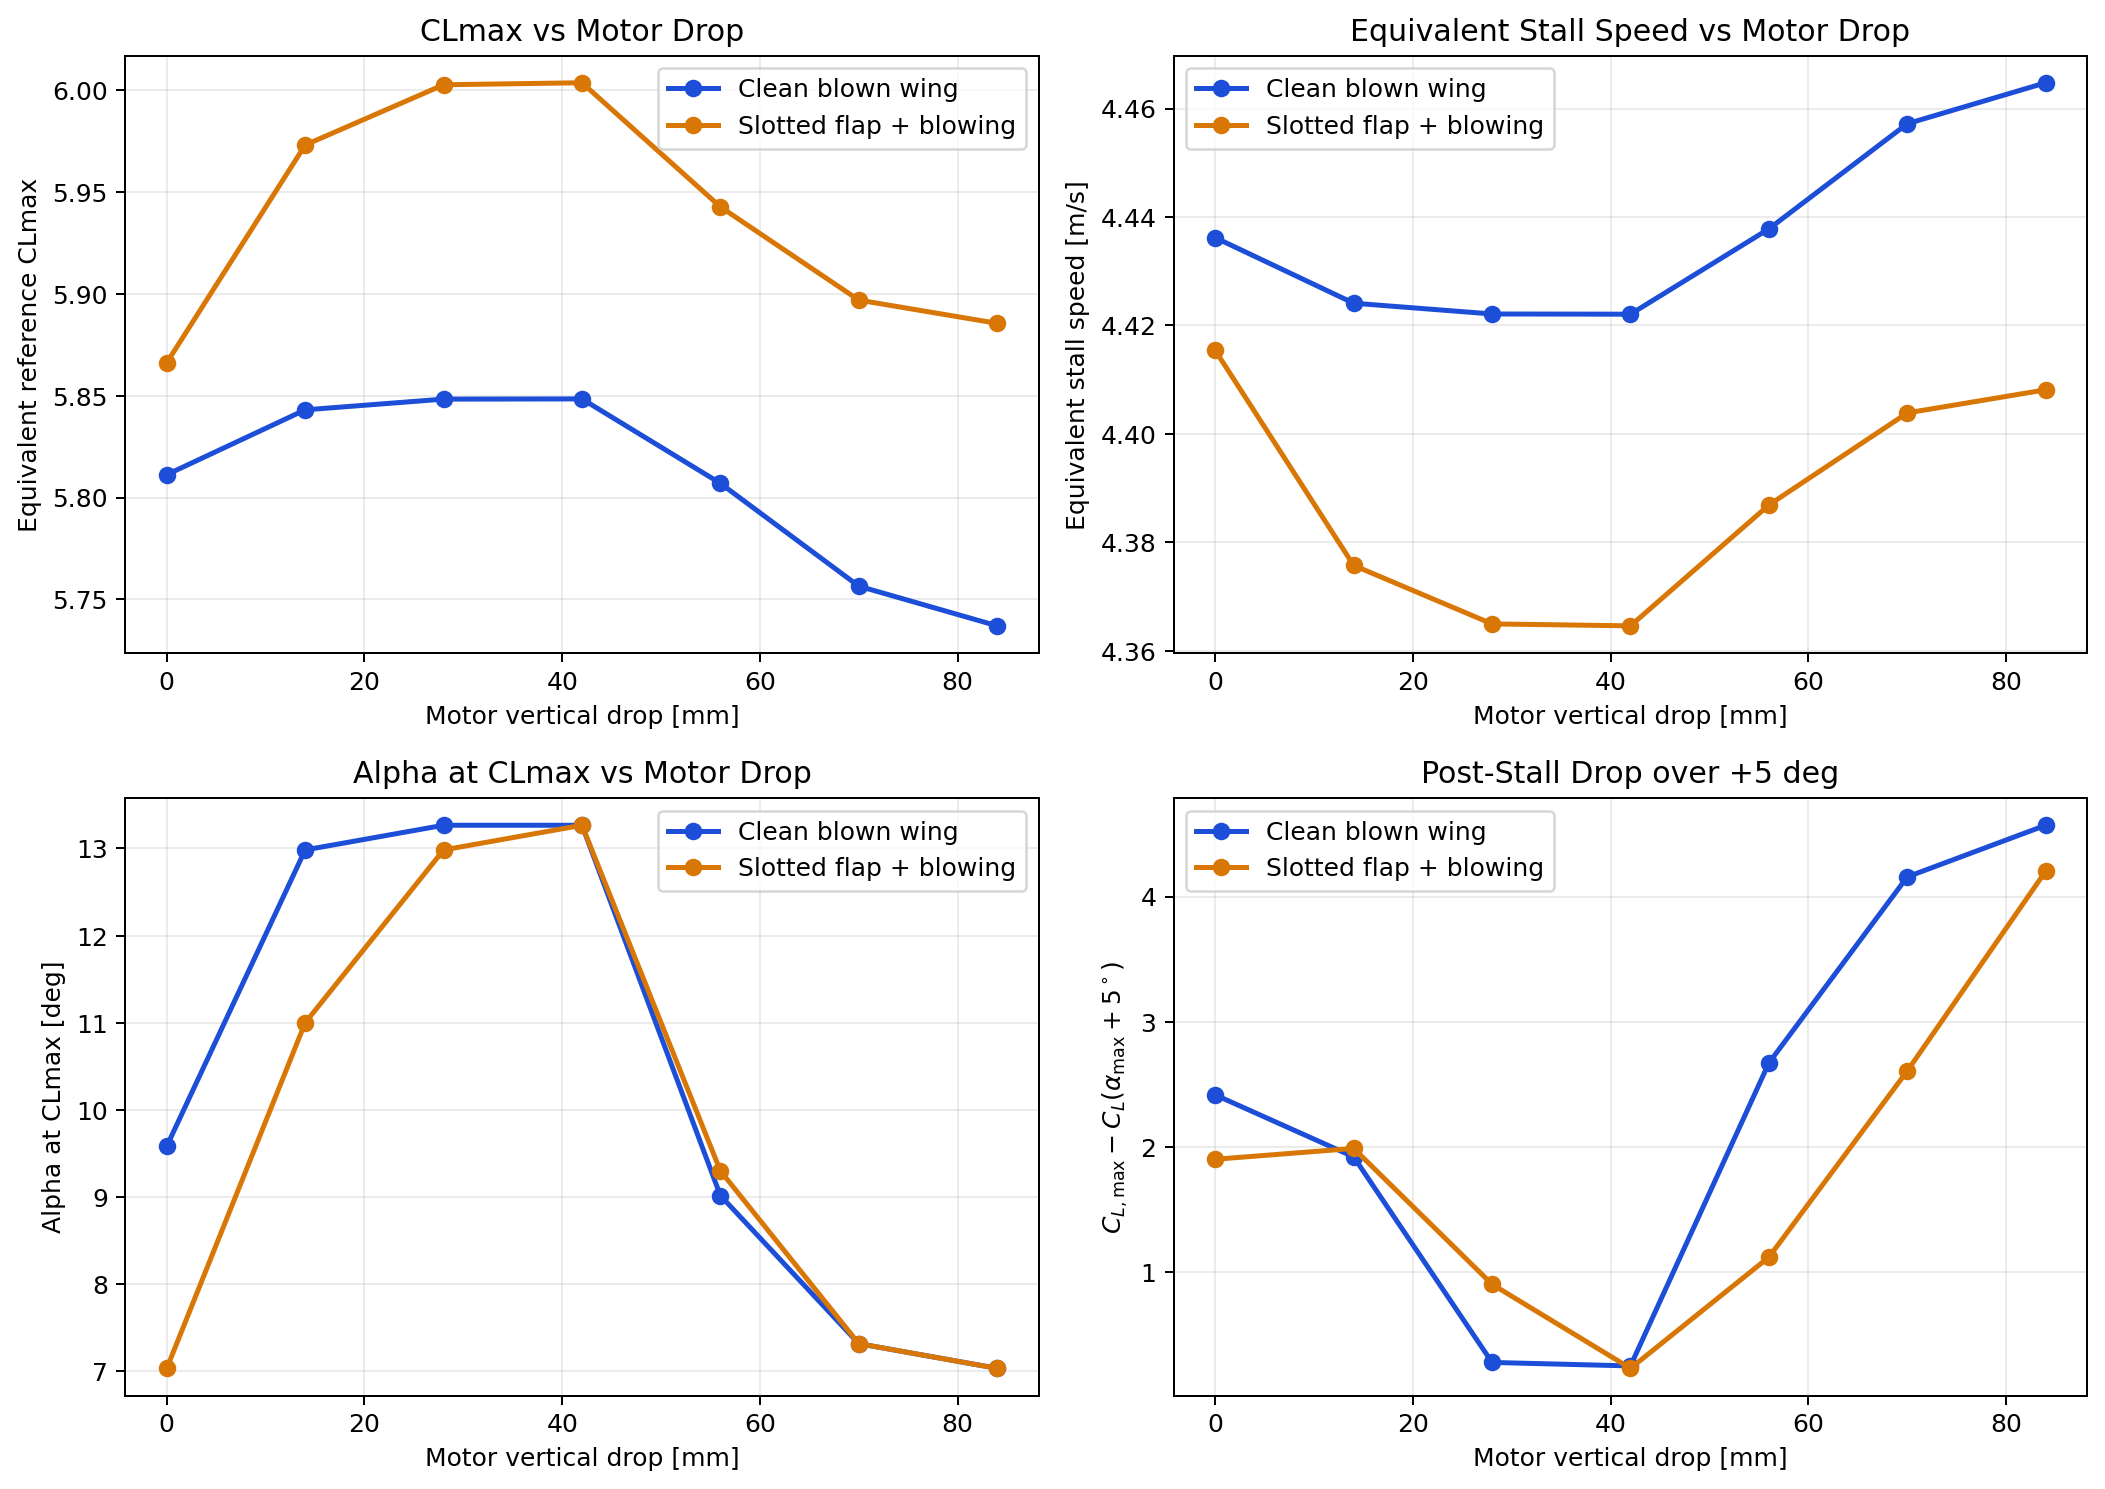
\includegraphics[width=0.92\linewidth]{../outputs/motor_height_trade/rank06_n10_d5p5_p2p2_balanced_b3/motor_height_trade_metrics.png}
    \caption{Motor-height trade metrics for the selected rank~6 architecture. Both the clean and flapped branches first improve with increasing drop, then plateau, then degrade as the over-drop penalty becomes active.}
    \label{fig:motor-metrics}
\end{figure}

\begin{figure}[H]
    \centering
    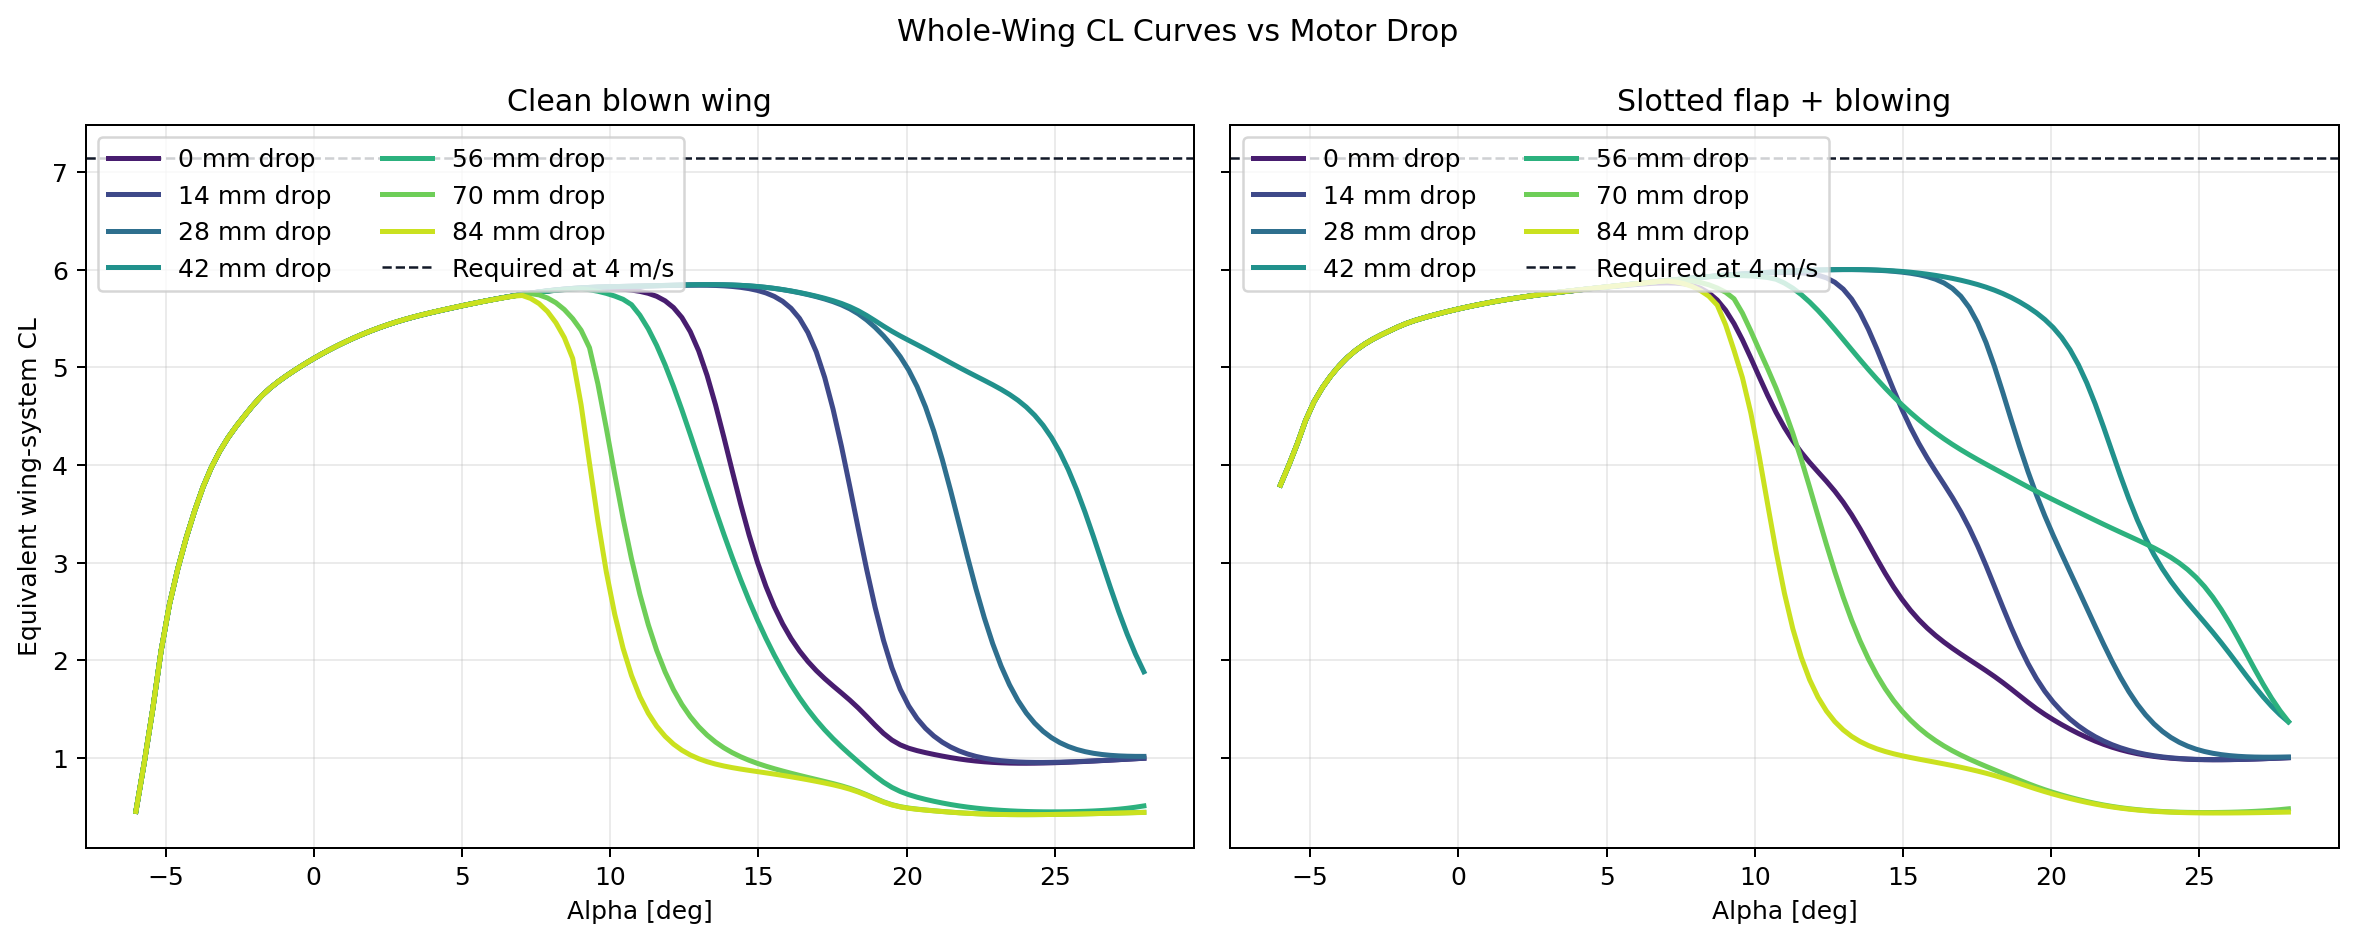
\includegraphics[width=0.92\linewidth]{../outputs/motor_height_trade/rank06_n10_d5p5_p2p2_balanced_b3/motor_height_trade_cl_overlay.png}
    \caption{Whole-wing \(C_L\) overlays for the clean-blown and slotted-flap-blown branches at multiple motor-drop values. The overly low motor positions do not simply reduce peak lift; they also make the post-stall decay substantially steeper.}
    \label{fig:motor-overlay}
\end{figure}

Numerically, the current trade gives the following representative results:
\begin{itemize}
\item clean blown wing at \(\Delta z_p/c = 0.12\): \(C_{L,\max}\approx 5.85\), \(V_s\approx \SI{4.42}{m/s}\),
\item slotted flap plus blowing at \(\Delta z_p/c = 0.12\): \(C_{L,\max}\approx 6.00\), \(V_s\approx \SI{4.36}{m/s}\),
\item neither branch meets the \SI{4.0}{m/s} target under the current assumptions.
\end{itemize}

The present project therefore supports a simple design statement: motor drop should be large enough to keep the flap/wing system immersed in the jet, but not so large that the stall behaviour becomes unacceptably abrupt.

\section{Operating-Point Implications and Representative Motor Targeting}

\subsection{What the current concept can do}

The present selected concept is now well enough defined to state its credible operating envelope under the current model:
\begin{itemize}
\item low-speed blown condition near \SI{4.36}{m/s} equivalent stall speed rather than the target \SI{4.0}{m/s},
\item cruise at \SI{10}{m/s} with electrical power near \SI{131}{W},
\item loiter energy near \SI{39.35}{Wh} for the current \SI{18}{min} requirement,
\item low-speed blown velocity margin of about \SI{5.15}{m/s} relative to the Stage~1 required value,
\item high-lift wing-only pitching moment near \(C_M=-0.90\) at the peak-lift point.
\end{itemize}

This is a very useful result. The selected architecture is not energetically struggling; it is high-lift limited. In other words, the current concept is already close to the energy and propulsion regime it needs, but still short of the low-speed aerodynamic requirement.

\subsection{Representative motor and ESC targets}

The repository now converts the selected Stage~1 operating point into a representative motor target sheet. For the selected rank~6 architecture, the present required per-motor values are:
\begin{align}
P_{\mathrm{shaft,peak}} &\approx \SI{11.6}{W}, \\
P_{\mathrm{elec,peak}} &\approx \SI{17.1}{W}, \\
I_{\mathrm{peak}} &\approx \SI{1.16}{A}, \\
K_V &\approx \SI{771}{rpm/V}.
\end{align}
The current target band is widened heuristically to about \SIrange{655}{886}{rpm/V}. The representative local dataset currently identifies a SunnySky A2212 \SI{1000}{Kv} class motor and an \SI{8}{A} BLHeli-S ESC class as the nearest class-level matches.

\begin{figure}[H]
    \centering
    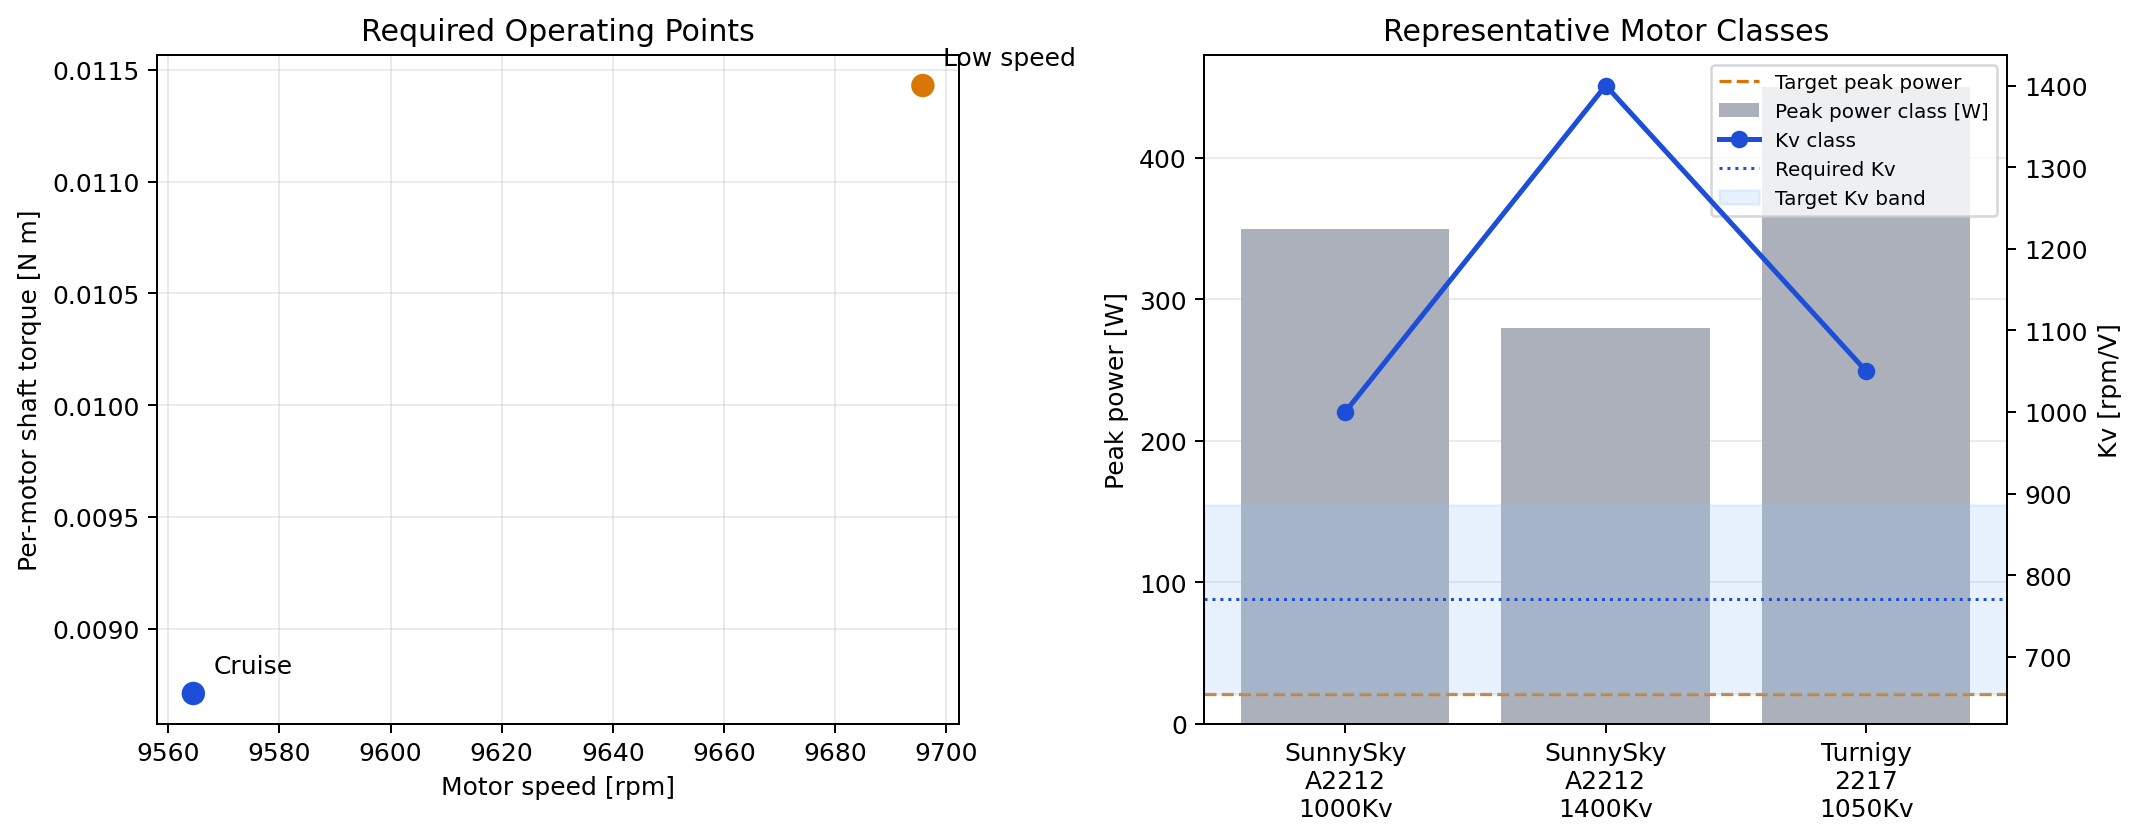
\includegraphics[width=0.92\linewidth]{../outputs/motor_targeting/rank06_n10_d5p5_p2p2_balanced_b3/motor_target_operating_points.png}
    \caption{Representative motor-targeting summary for the selected rank~6 architecture. The required operating point is modest, and the current local class dataset is much coarser and more heavily powered than the aerodynamic requirement itself. This is useful: it suggests that final hardware selection will not be limited by extreme power demand, but by packaging, mass, and availability.}
    \label{fig:motor-target}
\end{figure}

The important nuance is that these are not final part numbers. They are class-level proxies extracted from a local sizing dataset. The main conclusion is that the selected aerodynamic concept does not require an unusually large motor to be tested; the more serious remaining uncertainties are aerodynamic rather than electrical.

\section{Design Considerations for the Aircraft at the Present Stage}

The current repository is now mature enough to say something concrete about what the airplane should look like and what design moves remain most valuable.

\subsection{The propulsion concept}

The \(10\times 5.5\times 2.2\)~in balanced architecture remains a defensible study baseline because it combines:
\begin{itemize}
\item low cruise power relative to the rest of the Pareto set,
\item the highest momentum coefficient in the screened family,
\item enough propeller count to distribute blowing spanwise,
\item small enough diameter to package ten propellers on the \SI{2.0}{m} span.
\end{itemize}
This does not mean the concept is globally optimal. It means it is a good architecture around which to resolve the remaining aerodynamic questions.

\subsection{The wing}

The fixed-span geometry study suggests that the aerodynamic planform would prefer:
\begin{itemize}
\item somewhat larger wing area than the original \SI{0.70}{m^2} rectangular baseline,
\item moderate taper (\(\lambda \approx 0.62\)),
\item modest washout (about \(-2.5^\circ\)).
\end{itemize}
However, the control-surface study indicates that even the current rectangular wing with aggressive blown slotted flaps only reaches \(C_{L,\max}\approx 6.00\). This has an immediate implication: if \SI{4.0}{m/s} remains a hard mission requirement, either the wing must become larger, the mass must come down, or the local high-lift system must improve further.

Using the rectangular-wing control result,
\begin{equation}
S_{\mathrm{req}} \approx \frac{W}{q_\infty C_{L,\max}},
\end{equation}
the current \(C_{L,\max}\approx 6.0\) implies that the present \SI{5.0}{kg} airplane would require roughly
\begin{equation}
S_{\mathrm{req}} \approx \SI{0.83}{m^2}
\end{equation}
to hold \SI{4}{m/s}, which is about 19\% larger than the original rectangular wing and about 12\% larger than the current rank~6 Stage~3 refined wing. Conversely, keeping the original \SI{0.70}{m^2} wing but limiting the airplane to \(C_{L,\max}\approx 6.0\) implies a mass closer to \SI{4.2}{kg} if the \SI{4}{m/s} requirement is to be met. This is one of the clearest design outputs of the project.

\subsection{The high-lift system}

The selected flap is already large and strongly integrated with the propeller layout:
\begin{itemize}
\item \(65\%\) semispan,
\item \(c_f/c = 0.34\),
\item \(\delta_f = 40^\circ\),
\item overlap with 8 of the 10 propeller disks.
\end{itemize}
This means the project has already exhausted the most obvious ``just make the flap bigger'' move. Future improvements in low-speed capability are therefore more likely to come from improved section choice, improved slot geometry, better flap kinematics, or a modest increase in wing area than from merely extending the flap further.

\subsection{Motor height}

The present motor-height trade supports a drop near \(0.08c\) to \(0.12c\). That range is consistent with the paper-backed scale from Hawkswell et al. and with the present control study. There is no strong evidence in the current results that pushing the motor much lower than that is beneficial. Indeed, the present over-drop penalty suggests that such a change would likely sharpen stall before it helps the mean lift level.

\subsection{Controls and trim}

The current blown flap does not come for free. The wing-only pitching moment near the high-lift point is strongly negative, and the low-speed aileron authority, while still viable, is weaker than the cruise condition. The design implication is straightforward: the next aircraft-level study should not only optimize \(C_L\), but also ensure that the empennage and CG envelope can absorb the trim penalty associated with the blown slotted-flap system.

\section{Limitations and Recommended Next Steps}

The present workflow is coherent, but it is not the final answer. The main limitations are:
\begin{itemize}
\item Stage~1 propeller aerodynamics remain surrogate-based rather than tied to a specific measured propeller family.
\item The blown-strip response is paper-informed but not yet quantitatively fitted to a dedicated data set for the specific geometry being studied.
\item The motor-height over-drop penalty is qualitative, not experimentally fitted.
\item The rectangular-wing control study still uses a low-speed aileron proxy rather than a full lateral-directional model.
\item The representative motor target stage is class-based and uses local datasets rather than a live vendor-backed search.
\end{itemize}

The most valuable next steps are therefore:
\begin{enumerate}
\item replace the coarse Stage~1 propeller surrogates with measured propeller data for the candidate \(5.5\)~in and \(6.0\)~in classes,
\item calibrate the motor-height and blown-section surrogates directly against a section data set in the spirit of Agrawal et al.,
\item carry the flap-induced \(C_M\) burden into a whole-aircraft trim and tail-sizing study,
\item test whether modest increases in wing area or reductions in mass are a more efficient way to reach the \SI{4.0}{m/s} requirement than pursuing still more aggressive blown lift.
\end{enumerate}

\section{Conclusions}

This project has produced a usable, coherent design workflow for a blown-wing aircraft concept. The main findings are:
\begin{enumerate}
\item The Stage~1 Pareto optimizer is doing useful work. It is not merely sweeping propeller parameters; it is exposing the fundamental trade between cruise power, jet authority, and geometric coverage.
\item The selected \(10\times 5.5\times 2.2\)~in balanced architecture was retained for good reason. It sits near the low-cruise-power edge of the Pareto front while also preserving the highest momentum coefficient in the screened family, making it a strong candidate for downstream blown-wing study.
\item Large section \(c_l\) values from blown-flap literature should not be interpreted directly as whole-aircraft \(C_L\). Once the wing is assembled at common \(\alpha\), the present selected concept reaches a more realistic \(C_{L,\max}\approx 6.0\), not 8--9.
\item The present rectangular-wing study supports a large inboard single-slotted flap and a viable outboard aileron, but the concept still falls short of the \SI{4.0}{m/s} requirement under the current mass and wing area assumptions.
\item Motors in front of flaps matter not simply because they add momentum, but because they create a jet/flap system. That system increases lift, deepens the wing-only pitching moment, and makes motor height a genuine high-lift design variable.
\item The current motor-height trade is physically richer than the earlier bonus-factor model. It now captures both the benefit of recovering jet immersion and the degradation associated with overly aggressive motor drop.
\item The present operating point is not dominated by propulsion power or battery energy. The main challenge that remains is still low-speed aerodynamic capability and the trim burden that accompanies it.
\end{enumerate}

In that sense, the project has done what a good design-space study should do: it has narrowed the uncertainty. The current concept is not yet the final airplane, but it is now clear where the remaining leverage lies --- in wing area, mass, high-lift effectiveness, and trim --- and where it does not.

\section*{References}
\begin{thebibliography}{99}

\bibitem{Hawkswell2022}
Hawkswell, C., Romain, J., and Babinsky, H.,
``Selection of Propeller-Wing Configuration for Blown Wing Aircraft,''
\emph{AIAA SCITECH 2022 Forum},
AIAA Paper 2022-1024,
2022.

\bibitem{Agrawal2019}
Agrawal, S., Gaunaa, M., and Jameson, A.,
``Wind Tunnel Testing of a Blown Flap Wing,''
\emph{AIAA AVIATION 2019 Forum},
AIAA Paper 2019-3170,
2019.

\end{thebibliography}

\end{document}
